%\documentclass[final,authoryear,1p]{elsarticle}
%\documentclass[final,authoryear,5p,times,twocolumn]{elsarticle}
%\documentclass[authoryear,preprint,review,9pt]{elsarticle}
\documentclass[journal]{IEEEtran}
\usepackage{amssymb}
\usepackage{amsmath}
\usepackage{bbm}
\usepackage{graphicx}
\usepackage{subfig}
\usepackage{algorithmic}
\usepackage{algorithm}
\usepackage{relsize}
\usepackage{booktabs}
\usepackage{color}
\usepackage[labelfont={small,bf}]{caption}
\usepackage[font={small,bf}]{caption}
\usepackage[numbers]{natbib}
\renewcommand{\bibfont}{\footnotesize}
\usepackage[margin=0.6in]{geometry}
\newcommand{\closer}{\vspace{-0.0cm}}
\newcommand{\figcloser}{\vspace{-0.4cm}}

\begin{document}


%\begin{frontmatter}

\title{\huge Symmetric Diffeomorphic Registration with Expected Cross-Correlation for Multi-Modal Brain MRI}
\author{
    \IEEEauthorblockN{{\bf Omar Ocegueda}\IEEEauthorrefmark{1}}~\and~
    \IEEEauthorblockN{{\bf Eleftherios Garyfallidis}\IEEEauthorrefmark{2}}~\and~
    \IEEEauthorblockN{{\bf Maxime Descoteaux}\IEEEauthorrefmark{2}}~\and~
    \IEEEauthorblockN{{\bf Mariano Rivera}\IEEEauthorrefmark{1}}\\
    \IEEEauthorblockA{\IEEEauthorrefmark{1}Centro de Investigaci\'{o}n en Matem\'{a}ticas, Guanajuato, Gto, M\'{e}xico}\\
    \IEEEauthorblockA{\IEEEauthorrefmark{2}Computer Science Department, Universit\'{e} de Sherbrooke, Sherbrooke, Qu\'{e}bec, Canada}
}

%\author{Omar Ocegueda, Eleftherios Garyfallidis, Maxime Descoteaux~and~Mariano Rivera}
%\ead{jomaroceguedag@gmail.com}
%\cortext[cor1]{Corresponding author}

%\address[cimat]{, }
%\address[scil]{}
\maketitle
%\vspace{-1.0cm}
\begin{abstract}
    We present a new similarity measure for multi-modal brain MRI registration. The relationship between voxel intensities in both modalities is modeled as a global non-linear transfer function that makes their local \textcolor{blue}{intensity correspondence} as linear as possible. The proposed similarity measure results from a maximum-likelihood estimation of our model's parameters. We show that our functional is closely related to the local Cross Correlation metric and the optimal transfer function used in the Correlation Ratio. We implemented our similarity measure to drive the Symmetric Normalization (SyN) algorithm and compared its performance to traditional similarity metrics using real, publicly available, brain MR images. Quantitative results show that our proposal performs better than cross correlation and mutual information in the multi-modal case without reducing performance in the mono-modal case.
\end{abstract}

\begin{IEEEkeywords}
Multi-modal registration, Deformable registration, Diffeomorphic, Expectation maximization, Cross-correlation
\end{IEEEkeywords}

%\end{frontmatter}


\vspace{-0.5cm}
\section{Introduction}
The human brain has been a subject of extensive research by the medical image community with a wide range of objectives, from practical clinical applications like disease diagnosis and surgical planning, to addressing scientific questions related to its structure and function. The goal of brain image registration is to compute a transformation that brings images of the brain into anatomical correspondence. We can classify volumetric image registration methods according to two main criteria: a) the deformation model (linear/non-linear), and b) the similarity measure (mono-modal/multi-modal). Registration of images from different modalities (\emph{multi-modal} image registration) is a specially challenging task, since an appropriate similarity metric is harder to define in the multi-modal case than in the \emph{mono-modal} case. Multi-modal image registration has traditionally been constrained to linear methods: since registration of medical images of different modalities is almost exclusively applied to intra-subject image registration, it is often believed that there must exist a linear transformation that correctly brings them into correspondence. However, certain imaging modalities present severe distortions that cannot be accommodated by a linear model. Consider for example the case of Echo Planar Images (EPI), which suffer from distortions caused by magnetic field inhomogeneities \cite{Tournier2011, Andersson2003}. In Fig. \ref{fig:example_t1b0_problem} we show an example of two $B_{0}$ EPI images (from a dwMRI dataset) with opposite phase encode directions and a T1-weighted image from the same subject. The noticeable geometric distortions in the $B_{0}$ images are caused by differences in the magnetic susceptibility of different tissue types of the brain. These geometric distortions make their registration to the T1 image (even being from the same subject), a non-linear problem if these artifacts are not corrected beforehand \cite{Bhushan2015}. Although several correction methods have been proposed to correct geometric distortions in EPI \cite{Andersson2003, Holland2010, Ruthotto, Irfanoglu2015}, most of them require at least two images acquired with opposite phase-encode directions. If such extra images are not available, for example in data sets which were acquired without considering the need for correction, then the images cannot be corrected prior to registration with the T1. Despite the complexity of this registration task, it has a wide range of potential applications. Combining diffusion data with T1 MRI, for instance, has the potential of significantly improving tractography \cite{Smith2012, Girard2014}. Besides diffusion MRI, the development of non-linear multimodal registration methods has the potential to impact other image modalities, like functional MRI (which are also affected by susceptibility-induced geometric distortions), and intra-operative ultrasound images, which capture the deformation of the brain as a result of brain surgery \cite{Rivaz2015, DeNigris2012}.
\begin{figure}[t!]
%\centering
%    \subfloat[]{\label{fig:T1B0_task_example_b0_up}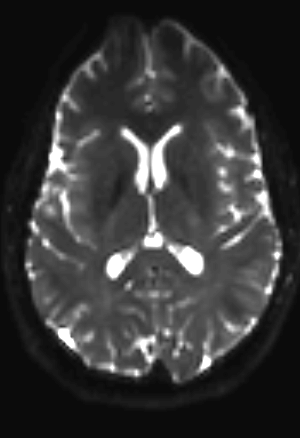
\includegraphics[width=0.3\linewidth]{./images/T1B0Result/T1B0_task_example_b0_up_enhanced.png}}
%    \subfloat[]{\label{fig:T1B0_task_example_b0_down}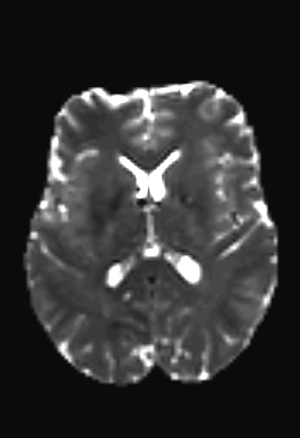
\includegraphics[width=0.3\linewidth]{./images/T1B0Result/T1B0_task_example_b0_down_enhanced.png}}
%    \subfloat[]{\label{fig:T1B0_task_example_t1}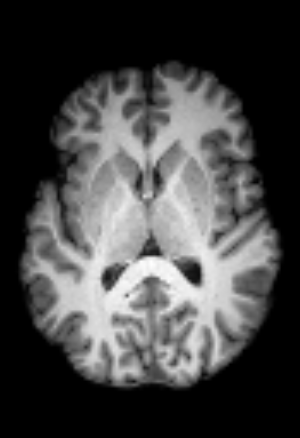
\includegraphics[width=0.3\linewidth]{./images/T1B0Result/T1B0_task_example_t1.png}}
%    \closer
%    \caption{{\small Two $B_{0}$ images with opposite phase-encode blips (a,b) and a T1 (c) from the same subject, acquired in the same session.}}
%\label{fig:example_t1b0_problem}\figcloser
%\end{figure}
\centering
    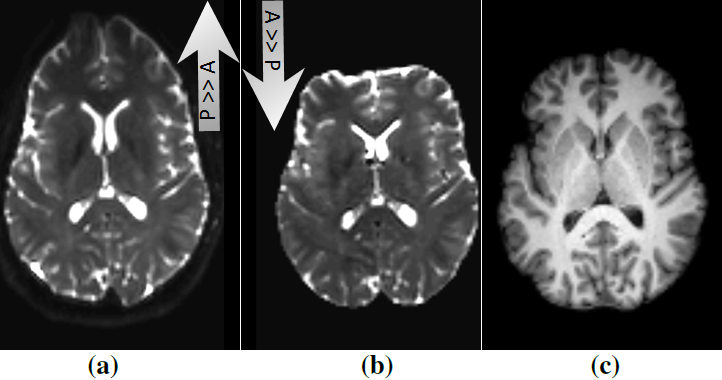
\includegraphics[width=1\linewidth]{./images/T1B0Result/figure1.png}
    \closer
    \caption{{\small Example of a multi-modal, non-linear, registration problem. (a,b) Two $B_{0}$ images with opposite phase-encode directions and (c) a T1-weighted image from the same subject. If both $B_{0}$ images are available, then the $B_{0}$ and T1-weighted images can be rigidly registered after the non-linear distortions have been corrected. However, if only one of the $B_{0}$ images is available, traditional correction algorithms are not applicable and co-registration of the distorted $B_{0}$ with the T1-weighted image is a non-linear registration problem.}}
\label{fig:example_t1b0_problem}\figcloser
\end{figure}
\vspace{-0.4cm}
\subsection{Information theoretic measures}
Existing multi-modal registration methods may be classified into two main approaches: 1) optimize information theoretic measures from the estimated joint probability distribution function (PDF), 2) reduce the multi-modal problem to the mono-modal case. The most prominent example of metrics based in information theory is mutual information (MI) \cite{Maes1997, Mattes2003}. The success of MI is explained by its generality, since it does not assume the existence of a functional relationship between the intensities in the two modalities. This generality comes at the expense of disregarding any notion of proximity of intensity values: two intensities will be considered similar only if their estimated joint PDF is high, no matter how close they are numerically, which may cause a large number of local maxima (see Fig. 2 in Roche {\it et al.}, 1998 \cite{Roche1998}). In the standard formulation of MI, the joint PDF is estimated from the whole image ({\it i.e.}, it is a {\it global} metric), which makes the metric more robust to the effects of noise \cite{Mattes2003}. An important limitation of this kind of global metrics is that the globally estimated PDF cannot capture non-stationary relationships between image intensities \cite{Hermosillo2004}. A direct approach to tackle this problem is to use locally estimated probability functions. Hermosillo {\it et al.} \cite{Hermosillo2004}, for instance, estimates the joint PDF locally by using Gaussian kernels centered at each voxel as weighting functions to reduce the contribution of far voxels. A limitation of this strategy, however, is its computational cost, as pointed out by Hermosillo \cite{Hermosillo2004}, since it results in a separate PDF estimation for each pixel, which makes it necessary to perform some simplifications. Besides, as we reduce the number of local samples, the estimation becomes more sensitive to noise~\cite{Mattes2003}.

\vspace{-0.2cm}
\subsection{Reduction to the mono-modal case}
Reducing the multi-modal problem to the mono-modal case may be accomplished by assuming the existence of a {\it transfer function} between the two modalities (a function that maps intensity values of one modality to corresponding intensities in the other). Although this strong assumption is not satisfied in general, experimental results have shown that it is not critical for typical brain image registration tasks~\cite{Roche1998}. Roche {\it et al.} \cite{Roche2000} showed that, assuming the existence of a transfer function, a maximum-likelihood formulation of the registration problem is equivalent to maximization of the correlation ratio (CR). Being a global metric, CR shares the robustness to noise of MI but also the inability to capture non-stationary relationships between image intensities. However, one of the advantages of CR over MI is that it is sensitive to proximity of intensity values, which may help to reduce the number of local maxima \cite{Roche1998}. An additional advantage is that CR can be computed efficiently from statistics from the images' iso-sets instead of explicitly estimating the joint PDF. Arce {\it et al.} \cite{Arce-santana2014} proposed a similar formulation of the registration problem which also makes the functional dependency assumption. In their work, the transfer function is modeled as a set of hidden random variables whose values can be estimated using the Expectation Maximization (EM) algorithm. Since the assumptions are similar to those made by Roche {\it et al.} \cite{Roche1998, Roche2000}, the resulting optimal transfer functions are the same. However, the resulting metric differs in that it introduces a measure of uncertainty for each intensity value, which helps to alleviate the effect of non-functional and non-stationary distributions. Recently, Bhushan {\it et al.} \cite{Bhushan2015} proposed an algorithm, called INVERSION, for T1-$B_{0}$ co-registration in the presence of susceptibility induced distortions. In their work, the $B_0$ to T1 transfer function is assumed to be monotonically decreasing and is computed by matching the intensity histograms of the input images. The main novelty of INVERSION is that the transfer function is applied to the $B_0$ after its intensities have been modulated with the local Jacobian of the transformation (eq. 5 in \cite{Bhushan2015}). However, since the transformation is not constrained to be diffeomorphic (as opposed to recent correction techniques \cite{Ruthotto, Irfanoglu2015}), the local Jacobian does not necessarily correspond to a transform explaining plausible geometric distortions \cite{Chang1992}. Also, since it is computed only from the histograms of the input images, the resulting transfer function may not be accurate enough, and the authors propose to refine the result using Normalized Mutual Information.

%One of the limitations of the original formulation proposed by Arce {\it et al.} \cite{Arce-santana2014} is that it is asymmetric (a limitation shared with CR) in the sense that the transfer function to be estimated must be chosen beforehand (to either map intensities from modality A to modality B or viceversa), which may result in very different solutions.
%Another limitation is that Arce {\it et al.} \cite{Arce-santana2014} use an elastic deformation model \cite{Bajcsy1982, Gee1999}, and their optimization strategy consists in a Gauss-Newton iterative algorithm \cite{GVK502988711} that requires to solve a series of large systems of linear equations.

\vspace{-0.2cm}
\subsection{Quantitative evaluation}
Validation is one of the most challenging aspects in image registration. The most accepted validation methodologies, in the mono-modal case, consist in measuring the overlap of manually annotated anatomical regions \cite{Klein2009, Klein2010, Rohlfing2012}. These methodologies have made possible to quantitatively evaluate non-linear registration algorithms and compare their performance in a meaningful way. However, to the best of our knowledge, there are no equivalent studies that quantitatively evaluate the accuracy of non-linear registration algorithms in the multi-modal case. In practice, performance is assessed only visually. The reason why validation becomes more challenging in the multi-modal case is that, as far as we know, there are no manually annotated multi-modal image sets publicly available.
%The Symmetric Normalization (SyN) algorithm developed by Avants {\it et al.} \cite{Avants2008, Avants2011}, and made available as part of the Advanced Normalization Tools (ANTS) %\cite{Avants2011a}, has been extensively tested in large comparative studies using the aforementioned methodologies and has consistently been reported as one of the most %accurate. For multi-modal images, the MI metric is implemented in ANTS, and can be used with SyN for diffeomorphic registration.

\vspace{-0.2cm}
\subsection{Summary of contributions}
Our contributions are two-fold:
\begin{enumerate}
\item{We propose a new matching functional for non-linear multi-modal brain MRI registration. Our model is based on the empirical observation (explained in detail in section \ref{sec:methods}) that the \textbf{non-linear, local} relationship between both modalities may be made closer to linear by applying a \textbf{global, non-linear} transfer function. We prove that the maximum likelihood estimator of the transfer function coincides (under mild assumptions) with the optimal transfer function used in the CR and EM functionals \cite{Roche1998} \cite{Arce-santana2014} \cite{Ocegueda2015}. The resulting functional, which we call Expected Cross Correlation (ECC) may be regarded as an extension to Cross Correlation (CC) to the multi-modal case. By estimating both transfer functions between image modalities, we eliminate the need for an image modality to be chosen {\it a priori}. Our symmetric formulation allows us to naturally implement our matching functional into the SyN \cite{Avants2011a} algorithm.}
\item{We propose a validation methodology for multi-modal brain MRI registration based on generating semi-synthetic images using a synthetic multi-modal template, and a set of real, manually annotated, brain images.}
\end{enumerate}
%This validation method obtained a Magna Cum Laude award at ISMRM 2015 anual meeting \cite{Ocegueda2015}.
%\footnote{A more precise name would be ``Squared Normalized Local Cross Correlation'', but it is more commonly known as simply ``Cross Correlation'' (see for example eq.(4) in \cite{Avants2008}).} 
\section{Background}

We regard an image $I$ as a function that maps voxels of a rectangular grid \hbox{$\mathcal{L}$}, of dimensions $n_{x} \times n_{y} \times n_{z}$ cells, to a set $G$ of
possible values called the ``dynamic range'' of $I$. The images we are interested in represent objects in physical space. This means that each point $(i,j,k)$ in the
3-dimensional grid $\mathcal{L}$ is associated to a point $(x,y,z) \in \Omega \subset \mathbf{R}^{3}$. The function that maps voxel coordinates of a grid $\mathcal{L}$ to their corresponding coordinates in physical space is an invertible affine transformation. Whenever we talk about
a grid $\mathcal{L}$ we implicitly assume that this $\mathcal{L}$ is associated to a specific grid-to-space affine transformation.
Since our images represent objects in physical space, and these objects are not tied to any specific grid, the same object may be sampled over any grid $\mathcal{L}$. Since
the grid-to-space transformation is invertible, we can, and will, unambiguously talk about images defined in physical space $\Omega \subset \mathbf{R}^{3}$.\\

\subsection{Matching functionals}
Defining an adequate similarity metric between two images $I, J$ defined over $\Omega_{I}$ and $\Omega_{J}$, respectively, is arguably the most important aspect of image registration, and has been the subject of significant amount of research \citep{Sotiras2013}, if the minimum of the metric does not coincide with what we understand by optimal image correspondence, then no matter what transformation or optimization algorithm we choose, we are unlikely to correctly align the images. In the mono-modal case, a plausible model describing the input images is given by
\begin{equation}\label{eq:ssd_model}
    I(v) = J(\phi(v)) + \eta(v), \; \forall v\in\Omega_{I}
\end{equation}
where the Gaussian random variables $\eta(v) \sim N(0, \sigma^{2})$ are assumed to be independent and identically distributed. Under these assumptions, the negative log-likelihood of the observed images is proportional to the Sum of Squared Differences (SSD), given by
\begin{equation}\label{eq:ssd_functional}
    SSD(I, J; \phi) = \sum_{v \in \Omega_{I}} \left(I(v) - J(\phi(v))\right)^{2}.
\end{equation}
Thus, minimization of \eqref{eq:ssd_functional} with respect to the transformation $\phi$ corresponds to a maximum likelihood estimation of the parameters of model \eqref{eq:ssd_model} (the parameters being the transformation $\phi$). There are two main limitations of model \eqref{eq:ssd_model} in the context of brain MRI: a) it does not take into account spatial intensity inhomogeneities and b) the functional is computed \emph{point-wise}, which makes it susceptible to noise and unable to capture local image features beyond one single voxel. To overcome these limitations, \cite{Wang2014} recently proposed a local linear model that attempts to account for the bias field in brain MRI. Let $W_{v} = \left\lbrace v_{1}, v_{2}, ..., v_{n} \right\rbrace$ be a rectangular local window centered at $v\in\Omega_{I}$, containing $n$ points and denote by $\mathbf{x_{v}} = (I(v_{1}), I(v_{2}), ..., I(v_{n}))^{T}$, $\mathbf{y_{v}} = (J(\phi(v_{1})), J(\phi(v_{2})), ..., J(\phi(v_{n})))^{T}$ the input images evaluated at all points $v_{i}\in W_{v}$, $i=1, ..., n$. Please keep in mind that $\mathbf{x_{v}}$ are fixed (they never change during optimization) while $\mathbf{y_{v}}$ change as we move $\phi$ (we cannot set the value of $\mathbf{y_{v}}$ freely but their value must be adjusted by moving $\phi$). Wang's local linear model states that, when $\phi$ correctly aligns $J$ to $I$, their intensities are approximately locally linear:
\begin{equation}\label{eq:wang_model}
    \mathbf{y_{v}} = \left[\mathbf{x_{v}} \; \mathbbm{1}\right]\beta + \eta(v) \; \forall v\in\Omega_{I}
\end{equation}
where $\mathbbm{1}$ is an $n$-vector whose entries are all equal to $1$,  $\beta = (\beta_{0}, \beta_{1})^{T}$ is the vector of $2$ parameters of the local linear model and the random vectors $\eta(v)\sim N(0, \sigma^{2} \mathbbm{I}_{n})$ are assumed to be independent and identically distributed, where $\mathbbm{I}_{n}$ is the $n \times n$ identity matrix. The maximum likelihood estimator for $\beta$ can be directly computed as
\begin{equation}\label{eq:wang_model_mle_beta}
    \widehat{\beta} =
    \left[\begin{array}{cc}
        \mathbf{x_{v}}^{T}\mathbf{x_{v}} & \mathbf{x_{v}}^{T}\mathbbm{1}\\
        \mathbf{x_{v}}^{T}\mathbbm{1} & n
    \end{array}\right]^{-1}
    \left[\begin{array}{c}
        \mathbf{x_{v}}^{T}\\
        \mathbbm{1}^{T}
    \end{array}\right]\mathbf{y_{v}}.
\end{equation}
By substituting $\beta = \widehat{\beta}$ in \eqref{eq:wang_model}, and summing over all points $v\in\Omega_{I}$ the negative log-likelihood is proportional to the ``local linear reconstruction'' (LLR) matching functional, proposed by \cite{Wang2014}:
\begin{equation}\label{eq:wang_metric}
    LLR(I, J;\phi) = \sum_{v\in\Omega_{I}}|| (\mathbf{P_{v}} - \mathbbm{I})\mathbf{y_{v}}||^{2},
\end{equation}
where
\begin{equation}\label{eq:def_P_v}
    \mathbf{P_v} = [\mathbf{x_{v}} \; \mathbbm{1}]
    \left[\begin{array}{cc}
        \mathbf{x_{v}}^{T}\mathbf{x_{v}} & \mathbf{x_{v}}^{T}\mathbbm{1}\\
        \mathbf{x_{v}}^{T}\mathbbm{1} & n
    \end{array}\right]^{-1}
    \left[\begin{array}{c}
        \mathbf{x_{v}}^{T}\\
        \mathbbm{1}^{T}
    \end{array}\right].
\end{equation}
The LLR matching functional turns out to be very robust for mono-modal registration. However, in some multi-modal registration tasks, the local linear model is insufficient to describe the relationship between image modalities. To exemplify this, figure \ref{fig:llr_test} depicts an example of the residual error of local linear reconstructions between two aligned brain images (a T1 and a T2 image) from the Brainweb dataset\footnote{The Brainweb dataset was used by \cite{Wang2014} in their evaluations.}. The center image in fig. \ref{fig:llr_test} depicts the reconstruction error in false color. Although the local relationship between both images is close to linear almost everywhere, there are local regions where the intensity relationship is not close to linear regardless of what image is selected as predictor (either T1 as a function of T2 or viceversa).\\

\begin{figure}[t!]
\centering
    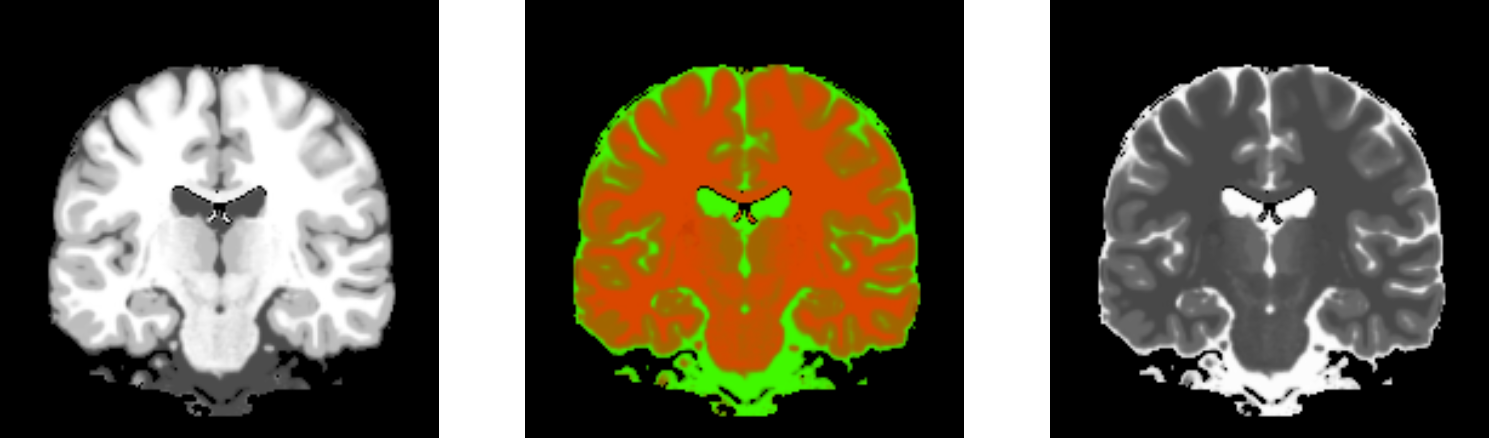
\includegraphics[width=1.0\linewidth]{./images/brainweb_t1_t2_overlay.png}\\
    \caption{Coronal slice of two realistic synthetic brain MRI images from the Brainweb dataset. The center image is an overlay of the T1 (left) image in the red channel, over the T2 (right) image in the green channel.}
\label{fig:brainweb_t1_t2}
\end{figure}

\begin{figure}[t!]
\centering
    \subfloat[]{\label{fig:T1T2_affine_fit_scatter1}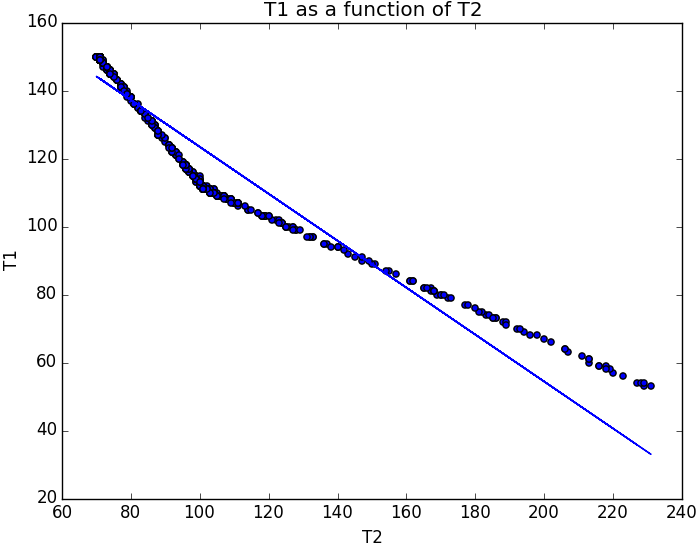
\includegraphics[width=0.2\linewidth]{./images/t1_aafo_t2_sample2.png}}
    \subfloat[]{\label{fig:T1T2_affine_fit_scatter2}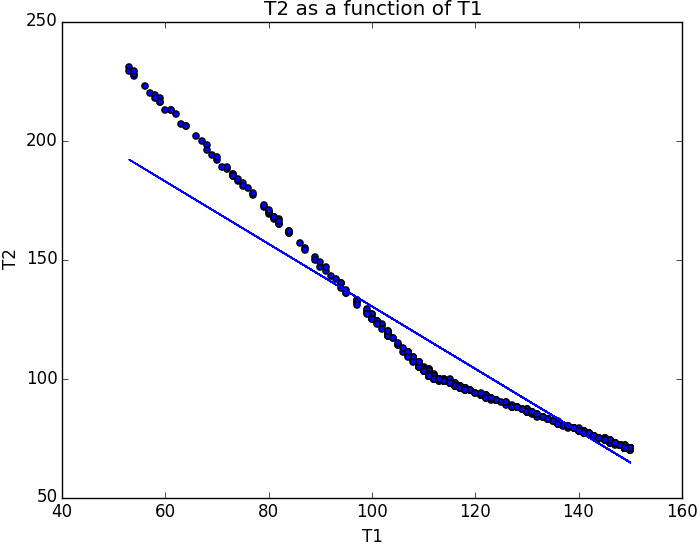
\includegraphics[width=0.2\linewidth]{./images/t2_aafo_t1_sample2.png}}
    \subfloat[]{\label{fig:T1T2_affine_fit_map}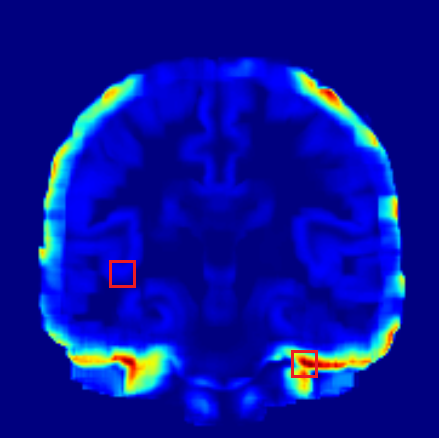
\includegraphics[width=0.2\linewidth]{./images/residuals_input.png}}
    \subfloat[]{\label{fig:T1T2_affine_fit_scatter1}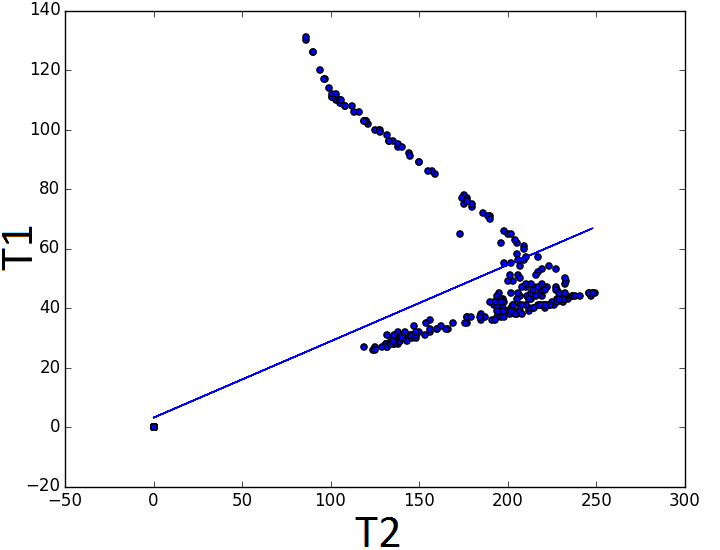
\includegraphics[width=0.2\linewidth]{./images/t1_aafo_t2_sample1.png}}
    \subfloat[]{\label{fig:T1T2_affine_fit_scatter2}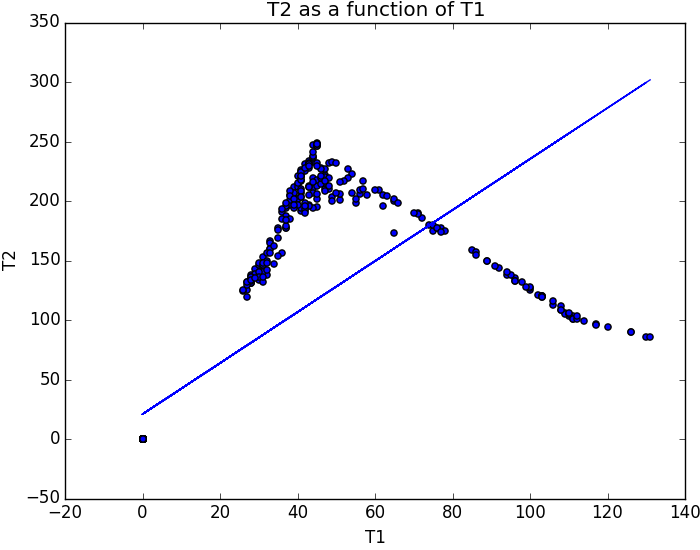
\includegraphics[width=0.2\linewidth]{./images/t2_aafo_t1_sample1.png}}\\
    \caption{Local linear reconstruction between intensities of a T1 and a T2 brain images (see fig. \ref{fig:brainweb_t1_t2}) under perfect alignment (Brainweb template). Center image (c) depicts the reconstruction error in false color (red means high reconstruction error and blue means low reconstruction error). Two local windows were selected: Left ( a)-b) ): a local window with a close-to-linear relationship between image intensities. Right (d) e) ): a local window with a non-linear relationship between image intensities. The scatter plots depict the best affine fit of T1 intensities as a function of T2 (a) and d) ), and the best fit of T2 as a function of T1 (b) and e)).}
\label{fig:llr_test}
\end{figure}

A more careful analysis of the LLR matching functional reveals that it is closely related to the popular Squared Normalized Local Cross Correlation metric, in the following sense. Note that we may assume, without loss of generality, that both vectors $\mathbf{x_{v}}, \mathbf{y_{v}}$ are \emph{centered} (i.e., their means are zero: $\frac{\mathbf{x_{v}}^{T}\mathbbm{1}}{n} = \frac{\mathbf{y_{v}}^{T}\mathbbm{1}}{n} = 0$), which may be proven as follows. Let's decompose $\mathbf{x_{v}}, \mathbf{y_{v}}$ into their centered part and their mean: $\mathbf{x_{v}} = \mathbf{x_{v}}' + \mu_{x}\mathbbm{1}$, and $\mathbf{y_{v}} = \mathbf{y_{v}}' + \mu_{y}\mathbbm{1}$, where $\mathbf{x_{v}}'$ and $\mathbf{y_{v}}'$ are centered. Then
\begin{displaymath}
    ||[\mathbf{x_{v}} \; \mathbbm{1}]\beta - \mathbf{y_{v}}||^{2} = ||[\mathbf{x_{v}}' \; \mathbbm{1}]\beta - \mathbf{y_{v}}' + \beta_{1}\mu_{x}\mathbbm{1} - \mu_{y}\mathbbm{1}||^{2} = ||[\mathbf{x_{v}}' \; \mathbbm{1}]\beta' - \mathbf{y_{v}}'||^{2}
\end{displaymath}
where $\beta' = (\beta_{1}, \beta_{0} + \beta_{1}\mu_{x} - \mu_{y})^{T}$. This $\beta'$ is the unique m.l.e. for $\beta$ in the centered case provided $\mathbf{x_{v}}$ is not a scalar multiple of $\mathbbm{1}$ (this condition makes the least squares system invertible, which makes the m.l.e. unique). This means that the LLR evaluated at non-centered vectors equals the LLR evaluated at their corresponding centered vectors. Let's consider the non-degenerate case first (the case where $\mathbf{x_{v}}$ is not a scalar multiple of $\mathbbm{1}$). In this case, as we previously showed, we can assume without loss of generality that $\mathbf{x_{v}}$ and $\mathbf{y_{v}}$ are centered. The projection matrix $\mathbf{P_{v}}$ in \eqref{eq:def_P_v} can be directly computed as
\begin{equation}\label{eq:projection_formula}
    \mathbf{P_{v}} = \frac{1}{\Delta}
    [\mathbf{x_{v}} \; \mathbbm{1}]
    \left[\begin{array}{cc}
        n & - \mathbf{x_{v}}^{T}\mathbbm{1}\\
        -\mathbf{x_{v}}^{T}\mathbbm{1} & ||\mathbf{x_{v}}||^{2}
    \end{array}\right]
    \left[\begin{array}{c}
        \mathbf{x_{v}}^{T}\\
        \mathbbm{1}^{T}
    \end{array}\right] =
    \frac{1}{n||\mathbf{x_{v}}||^{2}}
    [\mathbf{x_{v}} \; \mathbbm{1}]
    \left[\begin{array}{cc}
        n & 0\\
        0 & ||\mathbf{x_{v}}||^{2}
    \end{array}\right]
    \left[\begin{array}{c}
        \mathbf{x_{v}}^{T}\\
        \mathbbm{1}^{T}
    \end{array}\right]
\end{equation}
where $\Delta = n||\mathbf{x_{v}}||^{2} - \left(\mathbf{x_{v}}^{T}\mathbbm{1}\right)^{2} = n||\mathbf{x_{v}}||^{2} > 0$ ($||\mathbf{x_{v}}||^{2}$ cannot be zero, by hypothesis). Therefore, the entry $\mathbf{p_{i,j}}$ of $\mathbf{P_v}$ at row $i$, column $j$ is given by:
\begin{equation}
    \mathbf{p_{i,j}} = \frac{n\mathbf{x_{v}}_{i}\mathbf{x_{v}}_{j} + ||\mathbf{x_v}||^{2}}{n||\mathbf{x_{v}}||^{2}}.
\end{equation}
Each term of the LLR metric (corresponding to the local window centered at voxel $v$) can be writen as:
\begin{displaymath}
    ||(\mathbf{P_{v}} - \mathbbm{I})\mathbf{y_{v}}||^{2} = \sum_{i=1}^{n} \left(\sum_{j=1}^{n} \mathbf{p_{i,j}} \mathbf{y_{v}}_{j} - \mathbf{y_{v}}_{i}\right)^{2} =
    \sum_{i=1}^{n}\left(\frac{\mathbf{x_{v}}^{T}\mathbf{y_{v}}}{||\mathbf{x_{v}}||^{2}} \mathbf{x_{v}}_{i} - \mathbf{y_{v}}_{i}\right)^{2} = ||\mathbf{y_{v}}||^{2} - \frac{(\mathbf{x_{v}}^{T}\mathbf{y_{v}})^{2}}{||\mathbf{x_{v}}||^{2}} =
\end{displaymath}
\begin{equation}\label{eq:llr_cc_relationship}
    = ||\mathbf{y_{v}}||^{2}\left(1 - \frac{(\mathbf{x_{v}}^{T}\mathbf{y_{v}})^{2}}{||\mathbf{x_{v}}||^{2}||\mathbf{y_{v}}||^{2}}\right).
\end{equation}
Therefore, the LLR functional may be regarded as a modified Cross Correlation with a bias towards making $||\mathbf{y_{v}}||$ small (note that the CC metric operates on centered local vectors too). This bias may be removed from model \eqref{eq:wang_model} by normalizing $\mathbf{y_{v}}$:\\
\begin{equation}\label{eq:normalized_ll_model}
    \frac{\mathbf{y_{v}}}{||\mathbf{y_{v}}||} = \left[\mathbf{x_{v}} \; \mathbbm{1}\right]\beta + \eta(v) \; \forall v\in\Omega_{I},
\end{equation}
and we can see that maximization of likelihood under model \eqref{eq:normalized_ll_model} is now equivalent to maximization of the local cross correlation metric.\\

The matching functional we propose in this work is based on the empirical observation that, the non-linear relationship between both image modalities at local windows (illustrated in fig. \ref{fig:llr_test}) may be made closer to linear by applying a global, non-linear, transfer function $F: G \rightarrow \mathbbm{R}$ that maps intensities from one modality to the other. More precisely, our model may be written as
\begin{equation}\label{eq:ecc_model}
    \frac{\mathbf{y_{v}}}{||\mathbf{y_{v}}||} = \left[F\left[\mathbf{x_{v}}\right] \; \mathbbm{1}\right]\beta + \eta(v) \; \forall v\in\Omega_{I},
\end{equation}
where we have denoted $F[\mathbf{x_{v}}]$ the vector that results from applying function $F$ to each element of vector $\mathbf{x_{v}}$. By following the exact same steps as before, we can compute the optimal regression parameters $\widehat{\beta}$ and obtain the negative log-likelihood of our data under model \eqref{eq:ecc_model} (we just replace $\mathbf{x_{v}}$ with $F[\mathbf{x_{v}}]$ and $\mathbf{y_{v}}$ with $\frac{\mathbf{y_{v}}}{||\mathbf{y_{v}}||}$ in eq. \eqref{eq:llr_cc_relationship}):
\begin{equation}\label{eq:ecc_neg_likelihood}
    U(I, J;\phi) = \sum_{v\in\Omega_{I}}\left(1-\frac{\left(F\left[\mathbf{x_{v}}\right]^{T} \mathbf{y_{v}}\right)^{2}}{||F\left[\mathbf{x_{v}}\right]||^{2}||\mathbf{y_{v}}||^{2}}\right).
\end{equation}
The minimum of \eqref{eq:ecc_neg_likelihood} can be obtain by maximizing our proposed matching functional, which we call \emph{Expected Cross Correlation} (the reason of this name will be clear soon):
\begin{equation}\label{eq:ecc_functional}
    ECC(I, J;\phi) = \sum_{v\in\Omega_{I}}\frac{\left(F\left[\mathbf{x_{v}}\right]^{T} \mathbf{y_{v}}\right)^{2}}{||F\left[\mathbf{x_{v}}\right]||^{2}||\mathbf{y_{v}}||^{2}}.
\end{equation}
Now we will proceed to compute an optimal non-linear transfer function $F$. From model \eqref{eq:ecc_model}, the optimal function $F$ is not unique: if $F^{*}$ is optimal, then any affine transform of $F^{*}$, say $\widehat{F} = \alpha_{0} F^{*} + \alpha_{1}\mathbbm{1}$ is optimal too, because:
\begin{displaymath}
    \left[\widehat{F}\left[\mathbf{x_{v}}\right] \; \mathbbm{1}\right]\beta =
    \left[\left(\alpha_{0}F^{*}\left[\mathbf{x_{v}}\right]+\alpha_{1}\mathbbm{1}\right) \; \mathbbm{1}\right]\beta =
    \left[F^{*}\left[\mathbf{x_{v}}\right] \; \mathbbm{1}\right]\beta',
\end{displaymath}
where $\beta' = (\alpha_{0}\beta_{0}, \alpha_{1}\beta_{0} + \beta_{1})^{T}$. Therefore, what we want to find is the optimal $F$ modulo an affine transform. Let's denote by $m$ the number of different intensity values in the fixed image $I$ (a typical choice is $m=256$). We aim to assign a value $\mathbf{f}_{\ell}$ to each intensity $\ell$ of the fixed image, $0\leq \ell < m$, and define the transfer function $F$ as $F(\mathbf{x_{v}}_{i}) = \mathbf{f}_{\ell}$, where $\ell = \mathbf{x_{v}}_{i}$. The transfer function $F$ may then be represented as a vector $\mathbf{f}$ of dimension $m$. Let $\mathbf{k_{v}}_{\ell}$, and $\mathbf{a_{v}}_{\ell}$ be number of elements of $\mathbf{x_{v}}$ equal to $\ell$, and the sum of elements of $\mathbf{y_{v}}$ whose corresponding elements in $\mathbf{x_{v}}$ equal $\ell$, respectively. More precisely:
\begin{displaymath}
    \mathbf{k_{v}}_{\ell} = |\left\lbrace i : \mathbf{x_{v}}_{i}=\ell \right\rbrace|
\end{displaymath}
\begin{displaymath}
    \mathbf{a_{v}}_{\ell} = \sum_{i:\mathbf{x_{v}}_{i}=\ell} \mathbf{y_{v}}_{i}
\end{displaymath}
then, the dot product in equation \eqref{eq:ecc_neg_likelihood} may be written in term of $\mathbf{f}$ as follows:
\begin{displaymath}
    F\left[\mathbf{x_{v}}\right]^{T} \mathbf{y_{v}} = \sum_{\ell=1}^{m} \sum_{i:\mathbf{x_{v}}_{i}=\ell} F(\mathbf{x_{v}}_{i})\mathbf{y_{v}}_{i}
    =\sum_{\ell=1}^{m} \mathbf{f_{\ell}}\mathbf{a_{v}}_{\ell} = \mathbf{f}^{T}\mathbf{a_{v}}
\end{displaymath}
and the squared norm $||F[\mathbf{x_{v}}]||^{2}$ as:
\begin{displaymath}
    ||F\left[\mathbf{x_{v}}\right]||^{2} = \sum_{\ell=1}^{m} \sum_{i:\mathbf{x_{v}}_{i}=\ell} F(\mathbf{x_{v}}_{i})^{2}
    = \sum_{\ell=1}^{m} \mathbf{f_{\ell}}^{2} \mathbf{k_{v}}_{\ell} = \mathbf{f}^{T} \mathbf{D_{v}} \mathbf{f}
\end{displaymath}
where $\mathbf{D_{v}} = $ diag($\mathbf{k_{v}}$). Equation \eqref{eq:ecc_functional} can be written as:
\begin{equation}\label{eq:ecc_neg_likelihood_vector_form}
    ECC(I, J;\phi) = \sum_{v\in\Omega_{I}}\frac{\mathbf{f}^{T}\mathbf{a_{v}}\mathbf{a_{v}}^{T}\mathbf{f}}
    {\mathbf{f}^{T} \mathbf{D_{v}} \mathbf{f}||\mathbf{y_{v}}||^{2}}.
\end{equation}
The problem of maximizing the sum of quotients of quadratic forms, like eq. \eqref{eq:ecc_neg_likelihood_vector_form} doesn't have, in general, a close form solution, and it is necessary to resort to iterative algorithms (see for example \cite{Kiers1995} for a thorough review of this problem). The sole evaluation of the functional may be very time consuming because in order to apply fast strategies like partial sums (used for example by \cite{Avants2008} to evaluate the CC metric and its gradient) we need to store the partial results for each intensity value $0 \leq k < m$, which would require a very large amount of memory. Therefore, we will make a simplification based on the following assumptions. \\
1. The set of intensities of vector $\mathbf{x_{v}}$ are approximately a random sample from intensities of image $I$. Then, the number $\mathbf{k_{v}}_{\ell}$ of entries $i$ where $\mathbf{x_{v}}_{i}$ takes value $\ell$, may be approximated by its expected value $n\mathbf{p}_{\ell}$, where the probability $\mathbf{p}_{\ell}$ of a voxel having intensity $\ell$ may be estimated by the empirical probability:
\begin{equation}
    \mathbf{k_{v}}_{\ell} \approx \mathbbm{E}[\mathbf{k_{v}}_{\ell}] \approx n\frac{|\left\lbrace v\in\Omega_{I} : I(v) = \ell\right\rbrace|}{|\Omega_{I}|} = n\mathbf{p}_{\ell} 
\end{equation}

2. The average $\frac{\mathbf{a_{v}}_{\ell}}{n}$ of intensities of vector $\mathbf{y_{v}}$ whose corresponding entries in $\mathbf{x_{v}}$ are equal to $\ell$ may be approximated by the same average computed over the full image $J$, where intensities in $I$ are equal to $\ell$:
\begin{equation}
    \frac{\mathbf{a_{v}}_{\ell}}{n} =  \frac{1}{n}\sum_{i:\mathbf{x_{v}}_{i}=\ell} \mathbf{y_{v}}_{i} \approx \frac{1}{|\Omega_{I}|}\sum_{v\in\Omega_{I}: I(v)=\ell} J(\phi(v))
\end{equation}

Notice that, if the local windows $W_{v}, v\in\Omega{I}$ are sufficiently large, then these two conditions are, by definition, satisfied. The question is how small can we make the local windows so that these conditions are reasonably satisfied.

By making the change of variables $\mathbf{h_{v}} = \mathbf{D_{v}}^{\frac{1}{2}}\mathbf{f}$, we obtain:
\begin{equation}\label{eq:ecc_neg_likelihood_vector_form_simplified}
    ECC(I, J;\phi) = \sum_{v\in\Omega_{I}}\frac{\mathbf{h}^{T}\mathbf{D_{v}}^{-\frac{1}{2}}\mathbf{a_{v}}\mathbf{a_{v}}^{T}\mathbf{D_{v}}^{-\frac{1}{2}}\mathbf{h}}
    {\mathbf{h}^{T}\mathbf{h}||\mathbf{y_{v}}||^{2}}.
\end{equation}





















Before we proceed to the details on how to compute the optimal $F$, we illustrate the effect of incorporating a reasonable (not necessarily optimal according to model \eqref{eq:ecc_model}) global non-linear transfer into the local linear model. In this example, the fixed image $I$ is the T1, the moving image $J$ is the T2, and $F$ was chosen as the optimal transfer used in the Correlation Ratio metric (i.e. the average T2 intensity computed over iso-sets from the T1):
\begin{equation}\label{eq:cr_transfer}
    F(\ell) = \frac{1}{|G_{\ell}|}\sum_{v \in G_{\ell}} J(\phi(v))
\end{equation}
where $G_{\ell} = \left\lbrace v\in\Omega_{I}: I(v)=\ell\right\rbrace$ is the $\ell$-th iso-set of the fixed image $I$ . Fig. \ref{fig:ecc_test_good} depicts the same example as figure \ref{fig:llr_test}, but instead of fitting the local models between $I$ and $J$ directly, we used $F[I]$ and $J$. It can be observed that the non-linear local relationship was made significantly closer to linear by the use of the global transfer function.\\





\begin{figure}[t!]
\centering
    \subfloat[]{\label{fig:FT1T2_affine_fit_scatter1}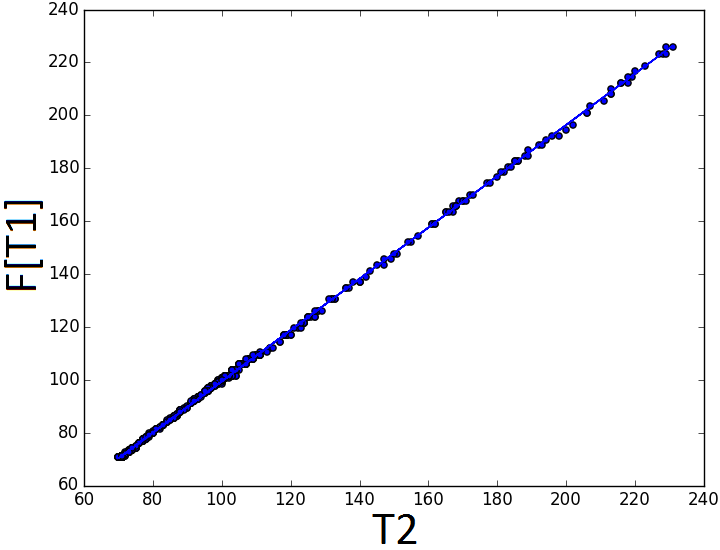
\includegraphics[width=0.2\linewidth]{./images/Ft1_aafo_t2_sample2.png}}
    \subfloat[]{\label{fig:FT1T2_affine_fit_scatter2}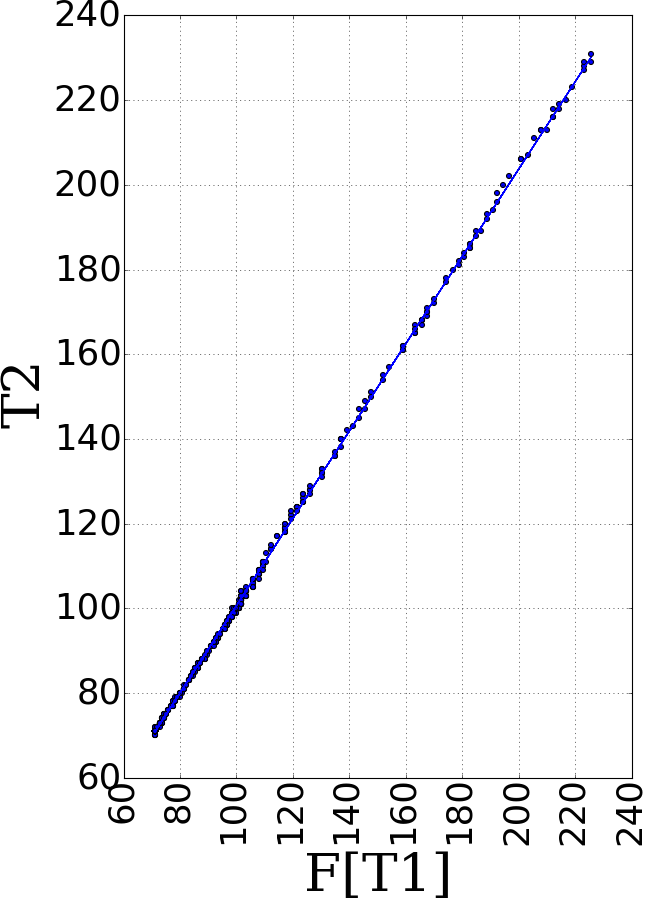
\includegraphics[width=0.2\linewidth]{./images/t2_aafo_Ft1_sample2.png}}
    \subfloat[]{\label{fig:FT1T2_affine_fit_map}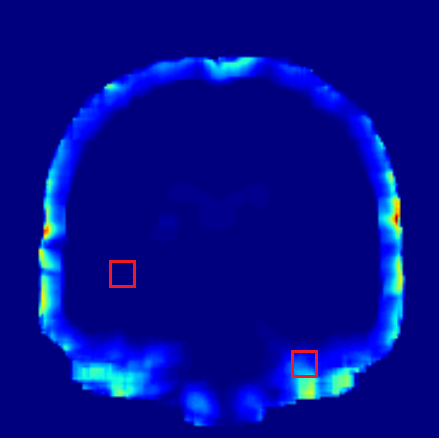
\includegraphics[width=0.2\linewidth]{./images/residuals_t2.png}}
    \subfloat[]{\label{fig:FT1T2_affine_fit_scatter1}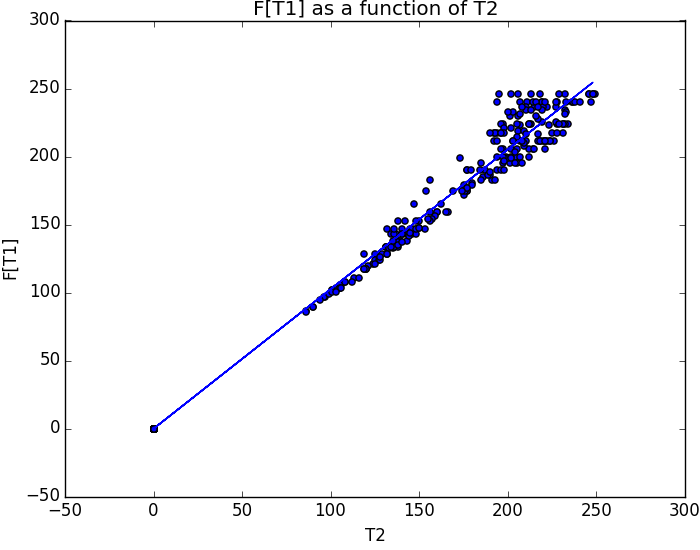
\includegraphics[width=0.2\linewidth]{./images/Ft1_aafo_t2_sample1.png}}
    \subfloat[]{\label{fig:FT1T2_affine_fit_scatter2}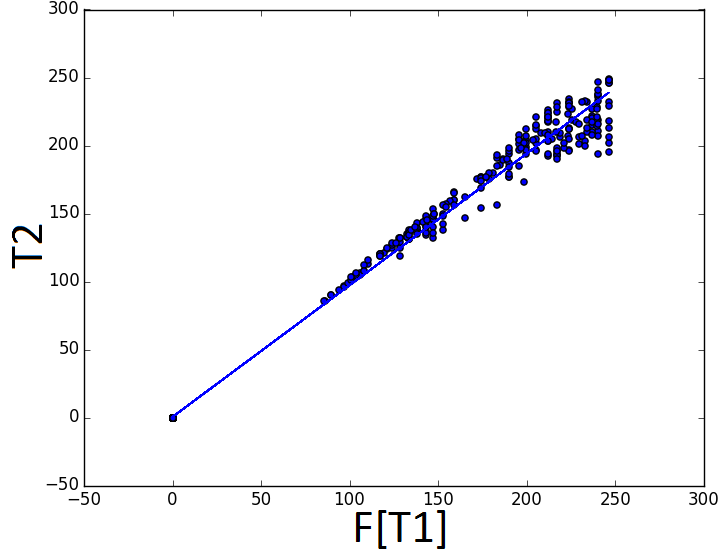
\includegraphics[width=0.2\linewidth]{./images/t2_aafo_Ft1_sample1.png}}\\
    \caption{Local linear reconstruction between T2 intensities and F[T1], where F is the global transfer function used in the Correlation Ratio metric (the average T2 intensity computed over iso-sets of the T1). Center image (c) depicts the reconstruction error in false color (red means high, and blue means low). The selected windows are the same as in figure \ref{fig:llr_test}. The scatter plots depict the best affine fit of F[T1] intensities as a function of T2 (a) and d) ), and the best fit of T2 as a function of F[T1] (b) and e)).}
\label{fig:ecc_test_good}
\end{figure}

A limitation of matching functionals that are based on the assumption of some kind of functional dependency between image intensities is that one of the image modalities must be chosen \emph{a priori} as the target modality (either map intensities from modality A to modality B or viceversa). This is an important decision and what choice is the best may not be obvious in general. Figure \ref{fig:ecc_test_bad} shows the same example as fig. \ref{fig:ecc_test_good}, but instead of mapping intensities from T1 to T2, we map intensities from T2 to T1. Although the transfer function from T2 to T1 helped, the relationship is still non-linear. Our matching functional considers both transfer functions, eliminating the need for a target modality to be chosen beforehand.\\

\begin{figure}[t!]
\centering
    \subfloat[]{\label{fig:T1FT2_affine_fit_scatter1}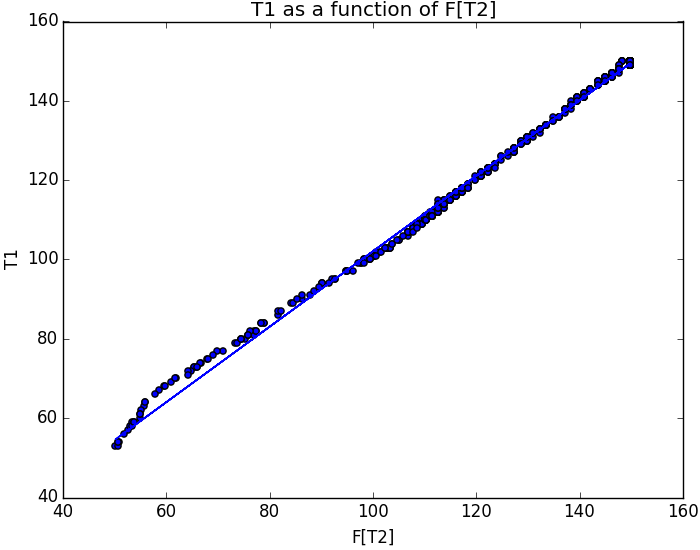
\includegraphics[width=0.2\linewidth]{./images/t1_aafo_Ft2_sample2.png}}
    \subfloat[]{\label{fig:T1FT2_affine_fit_scatter2}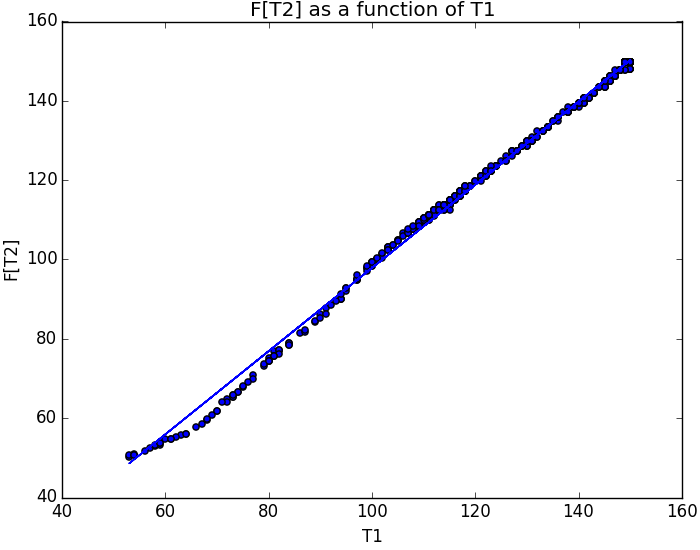
\includegraphics[width=0.2\linewidth]{./images/Ft2_aafo_t1_sample2.png}}
    \subfloat[]{\label{fig:T1FT2_affine_fit_map}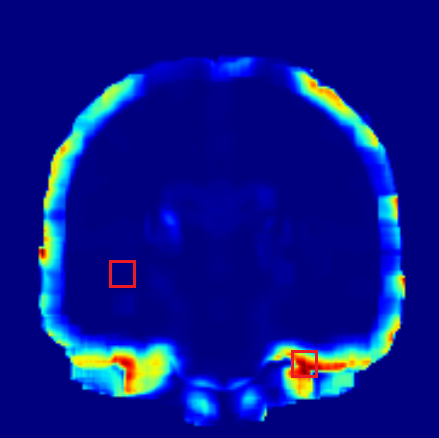
\includegraphics[width=0.2\linewidth]{./images/residuals_t1.png}}
    \subfloat[]{\label{fig:T1FT2_affine_fit_scatter1}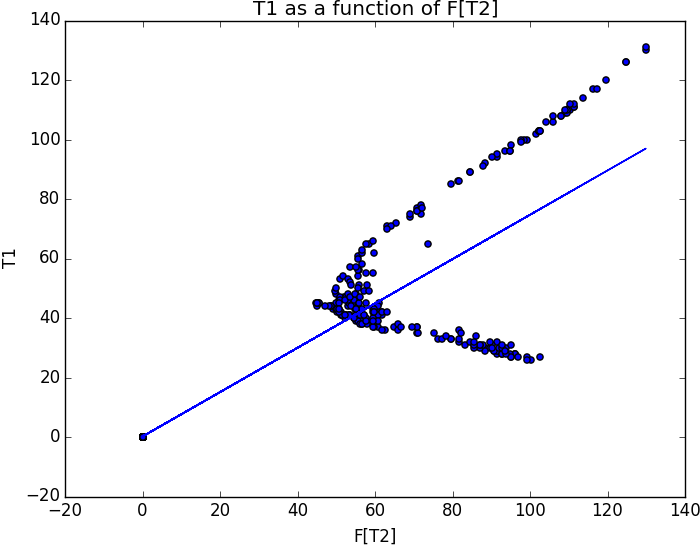
\includegraphics[width=0.2\linewidth]{./images/t1_aafo_Ft2_sample1.png}}
    \subfloat[]{\label{fig:T1FT2_affine_fit_scatter2}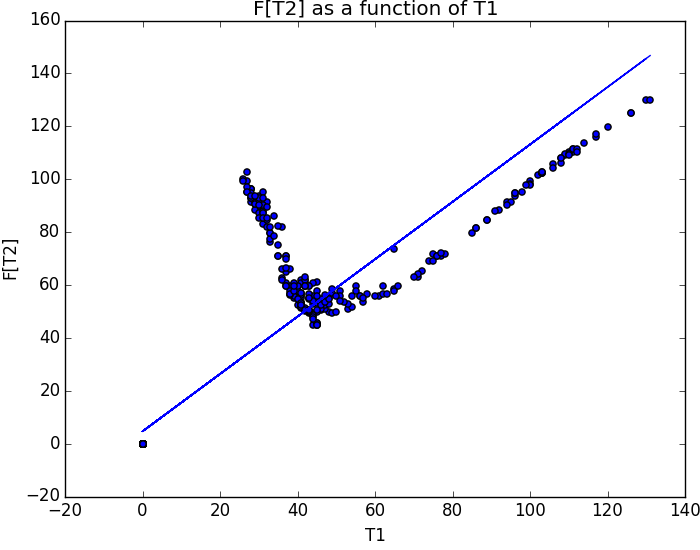
\includegraphics[width=0.2\linewidth]{./images/Ft2_aafo_t1_sample1.png}}\\
    \caption{.}
\label{fig:ecc_test_bad}
\end{figure}







To overcome these limitations, Cross-Correlation (CC) \footnote{Local Squared Normalized Cross Correlation would be a more precise name, but it is commonly called, for simplicity, Cross Correlation since it is clear in the context of non-linear registration that the correlation is computed within local windows and it is normalized and squared (see for example eq. (4) of \cite{Avants2008}).} does not assume that the intensities of the input images match poin twise and it is defined over local windows as follows. Denote by
\begin{equation}\label{eq:cc_functional}
    CC(I, J; \phi) = \sum_{x \in \Omega_{I}} \frac{}{||||}.
\end{equation}




is known to perform well in a larger number of applications since it compares local neighborhoods (as opposed to single voxel values used by SSD), which allows us to implicitly compare beyond voxel-level features. To understand how this is done, let's consider the following model\\

Recently, \cite{Arce-santana2014} modeled the transfer function between the image modalities as
\begin{equation}\label{eq:arce_model}
    F[I(x)] = J(\phi(x)) + \eta(x), x\in \mathcal{L}
\end{equation}
where $F$ is the (unknown) transfer function between image modalities and $\eta(x), x\in \mathcal{L}$ are independent random variables with Gaussian distribution. Since the grid $\mathcal{L}$ is discrete, image $F[I(x)], x\in \mathcal{L}$ may be modeled as a discrete set of hidden random variables $Y(x) = F[I(x)]$ whose distribution parameters
can be estimated using the Expectation Maximization (EM) algorithm \citep{Dempster1977}. In their work, \cite{Arce-santana2014} used a discretized elastic
deformation model to test the behavior of their metric, which leads to the following energy minimization problem

\begin{equation}\label{eq:arce_elastic}
    \mathbf{u}^{*} = \arg \min_{\mathbf{u}} \sum_{x \in \mathcal{L}} \frac{1}{2 \sigma(x)^{2}} ( \bar{I}(x) - J(x + \mathbf{u}(x)))^{2} + \lambda \sum_{<x, y>} ||\mathbf{u}(x) - \mathbf{u}(y)||^{2},
\end{equation}
where $\bar{I}(x), \sigma(x), x\in \mathcal{L}$ are the estimated parameters (mean and standard deviation) of the hidden variable $F[I(x)]$ given the
observed intensity $I(x)$ and $<x, y>$ denote neighboring pixels in $\mathcal{L}$. Even though the authors only evaluated their metric for 2D image registration and used
the elastic model, this formulation can be extended, as we will show in the next section, to develop an efficient and accurate symmetric diffeomorphic non-linear registration algorithm for 3D multi-modal images by taking advantage of the ideas of Avants' \textit{Greedy SyN} \citep{Avants2008}, Vercauteren's \textit{Diffeomorphic Demons} \citep{Vercauteren2009} and Arce's \textit{EM transfer function} model \citep{Arce-santana2014}.

\subsection{Symmetric diffeomorphic registration}

The goal of image registration is to compute a transformation $\phi: \Omega \rightarrow \Omega$ that brings a moving image $J:\Omega \rightarrow G$ into correspondence
with a fixed image $I:\Omega \rightarrow G$. The transformation $\phi$ is chosen from a set $\Phi$ of feasible solutions having properties that are desirable depending on the
application, such as smoothness and invertibility. Correspondence between $I$ and $J$ is defined to be reached when a dissimilarity metric between them is minimized.\\

In non-linear image registration, the transformation $\phi$ is usually represented by a deformation field $\mathbf{u(\cdot)}$ that assigns a displacement vector
to each point $x$ such that $\phi(x) = x + \mathbf{u}(x)$. The classical elastic model is one of the earliest formulation for non-linear image registration \citep{Bajcsy1982, Gee1999},
and may be written as

\begin{equation}\label{eq:elastic}
    \mathbf{u}^{*} = \arg \min_{\mathbf{u}} \int_{\Omega} ||L \mathbf{u}(x)||^{2}dV + \Pi(I, J \circ \phi),
\end{equation}
where $L$ is a differential operator used to promote smoothness on $\mathbf{u}$ and $\Pi$ is the dissimilarity metric driving the registration. A limitation of this model, especially important for medical image registration is that the solution, although being smooth, is not guaranteed to be invertible, and the topology of the moving image is not guaranteed to be preserved after transforming it under $\phi$.\\

To overcome the limitations of the elastic model, the large deformation proposed by \cite{Christensen2001} and further developed by \cite{Science2005} formulates the problem in terms of a trajectory of transformations \hbox{$\phi:\Omega_{I} \times [0, 1] \rightarrow \Omega_{J}$} that satisfies $\frac{d \phi(x, t)}{dt} = v(\phi(x, t), t)$ and $\phi(x, 0) = x$, where $v(\cdot, \cdot)$ is
the velocity field associated to the curve $\phi$. Beg's Large Deformation Diffeomorphic Metric Mapping (LDDMM) \citep{Science2005} formulation of the registration problem is given by:
\begin{equation}\label{eq:LDDMM}
    v^{*} = \arg \min_{v:\dot{\phi} = v_{t}(\phi)} \int_{0}^{1} ||L v_{t}||^{2} dt + \Pi(I, J \circ \phi(\cdot, 1)),
\end{equation}
where $\dot{\phi} = \frac{d\phi}{dt}$, $v_{t} = v(\cdot, t), t\in [0, 1]$. The final diffeomorphisms can be obtained by integrating over time
\begin{equation}\label{eq:velocity_integral}
    \phi(x, 1) = \phi(x, 0) + \int_{0}^{1}v(\phi(x, t), t) dt.
\end{equation}

\cite{Dupuis1998} showed that by enforcing sufficient smoothness in $v$, through the differential operator $L$, it can be guaranteed that $\phi(\cdot, t), t \in [0, 1]$ are diffeomorphisms. This and other formulations also based on diffeomorphic flows ensure that images are smoothly transformed and their topology preserved: an important property for many medical applications. \cite{Avants2008, Avants2011} modified the standard LDDMM formulation to enforce symmetry in the sense that the registration result is the same regardless of which image we designate as $I$ and $J$. This property, although natural and desirable, is not ensured in standard computational methods solving the LDDMM problem. By splitting the trajectory $\phi$ into two trajectories with opposite direction $\phi_{1}(x, t) = \phi_{2}(y, 1-t)$, where $y = \phi(x, 1)$, with corresponding velocity fields $v_{1}, v_{2}$, the Symmetric formulation for Diffemorphic Image Registration \citep{Avants2008, Avants2011} can be written as:

\begin{equation}\label{eq:syn_energy}
    \begin{array}{lll}
        v_{1}^{*}, v_{2}^{*} &=& \mathlarger{\arg \min \int_{t=0}^{0.5} ||L v_{1}(x, t)||^{2} + ||L v_{2}(x, t)||^{2} dt}\\
        &+& \mathlarger{ \Pi(I \circ \phi_{1}(\cdot, 0.5), J(\phi_{2}(\cdot, 0.5)))}
    \end{array}
\end{equation}
subject to
\begin{equation}\label{eq:syn_energy_constraints}
    \begin{array}{l}
        \frac{d\phi_{i}(x, t)}{dt} = v_{i}(\phi(x,t),t)\\
        \phi_{i}(\cdot, 0) = \mathbf{I},\, \phi_{i}^{-1}(\phi_{i}) = \mathbf{I},\, \phi_{i}(\phi_{i}^{-1}) = \mathbf{I},\, i=1,2,
    \end{array}
\end{equation}
where $\mathbf{I}$ denotes the identity transformation. \cite{Avants2006} proposed a numerical algorithm, called \textit{Geodesic SyN} for solving \eqref{eq:syn_energy}, which deforms both images towards the midpoint of the trajectory. The main drawback of directly solving eq. \eqref{eq:syn_energy} is its computational cost, since it requires space and time discretization and it is necessary to integrate the velocity fields in eq. \eqref{eq:velocity_integral} to obtain the trajectories at each iteration. A more efficient optimization algorithm to approximately solve eq. \eqref{eq:syn_energy}, also proposed by \cite{Avants2008, Avants2011}, consists in computing the gradient of the metric only at the midpoint of the trajectory (as opposed to evaluating it for all time):
\begin{equation}\label{eq:grad_metric}
    \nabla_{\phi_{i}} \Pi(\tilde{I}, \tilde{J}) = \frac{\partial}{\partial \phi_{i}} \Pi \left( \tilde{I}, \tilde{J}\right),
\end{equation}
where $\tilde{I} = I \circ \phi_{1}^{-1}(\cdot, 0.5)$, $\tilde{J} = J \circ \phi_{2}^{-1}(\cdot, 0.5)$. The midpoint diffeomorphisms are then updated by composition with the gradient after smoothing with a Gaussian kernel $K_{\sigma}$ (as opposed to integrating along the full geodesic)

\begin{equation}\label{eq:gsyn_update}
    \phi_{i}(\cdot, 0.5) = \phi_{i}(\cdot, 0.5) - \left( \epsilon K_{\sigma} \ast \nabla_{\phi_{i}} \Pi(\tilde{I}, \tilde{J}) \right) \circ \phi_{i}(\cdot, 0.5),
\end{equation}
where $\ast$ denotes the convolution operator and $\epsilon$ is a small factor controlling the step size in the optimization process. Finally, the updated midpoint transformations (which, after composition with the gradient, are not ensured to be diffeomorphisms) are forced to be invertible by using an explicit vector field inversion algorithm \citep{Chen2008}. This algorithm, called \textit{Greedy SyN} (see Appendix \ref{ap:Algorithms}, alg. \ref{alg:Greedy_SyN}) has been adopted by the neuroimaging community as the \textit{de facto} state-of-the-art brain MRI registration algorithm due to its reliability and efficiency. It was the method used for evaluating ANTS \citep{Avants2011} in the large comparative studies developed by \cite{Klein2009, Klein2010} in which \textit{Greedy SyN} consistently ranked first.



\vspace{-0.5cm}
\section{Methods}
A more detailed analysis of the LLR matching functional reveals that it is closely related to the CC metric, in the following sense. Let's consider the non-degenerate case first (the case that $\mathbf{y}_{v}$ and $\mathbf{x}_{v}$ are not ``constant'' vectors or in other words, they are not scalar multiples of $\mathbbm{1}$), we will discuss the degenerate cases later. First of all, note that we may assume, without loss of generality, that both vectors $\mathbf{x}_{v}, \mathbf{y}_{v}$ are \emph{centered} (i.e., their means are zero: $\frac{\mathbf{x}_{v}^{T}\mathbbm{1}}{n} = \frac{\mathbf{y}_{v}^{T}\mathbbm{1}}{n} = 0$), which may be proven as follows. Let's decompose $\mathbf{x}_{v}, \mathbf{y}_{v}$ into their centered part and their mean: $\mathbf{x}_{v} = \mathbf{x}_{v}' + \mu_{x}\mathbbm{1}$, and $\mathbf{y}_{v} = \mathbf{y}_{v}' + \mu_{y}\mathbbm{1}$, where $\mathbf{x}_{v}'$ and $\mathbf{y}_{v}'$ are centered. Then
\begin{displaymath}
    \begin{array}{lcl}
        ||[\mathbf{x}_{v} \; \mathbbm{1}]\beta - \mathbf{y}_{v}||^{2} &=& ||[\mathbf{x}_{v}' \; \mathbbm{1}]\beta - \mathbf{y}_{v}' + \beta_{1}\mu_{x}\mathbbm{1} - \mu_{y}\mathbbm{1}||^{2}\\
        &=&||[\mathbf{x}_{v}' \; \mathbbm{1}]\beta' - \mathbf{y}_{v}'||^{2}
    \end{array}
\end{displaymath}
where $\beta' = (\beta_{1}, \beta_{0} + \beta_{1}\mu_{x} - \mu_{y})^{T}$. This $\beta'$ is the unique m.l.e. for $\beta$ in the centered, non-degenerate case. This means that the LLR evaluated at non-centered vectors equals the LLR evaluated at their corresponding centered vectors. The projection matrix $\mathbf{Q}_{v}$ in \eqref{eq:def_P_v} can be directly computed as
\begin{align*}
    \mathbf{Q}_{v} &= \frac{1}{\Delta}
    [\mathbf{x}_{v} \; \mathbbm{1}]
    \left[\begin{array}{cc}
        n & - \mathbf{x}_{v}^{T}\mathbbm{1}\\
        -\mathbf{x}_{v}^{T}\mathbbm{1} & ||\mathbf{x}_{v}||^{2}
    \end{array}\right]
    \left[\begin{array}{c}
        \mathbf{x}_{v}^{T}\\
        \mathbbm{1}^{T}
    \end{array}\right] \\
    &= [\mathbf{x}_{v} \; \mathbbm{1}]
    \left[\begin{array}{cc}
        \frac{1}{||\mathbf{x}_{v}||^{2}} & 0\\
        0 & \frac{1}{n}
    \end{array}\right]
    \left[\begin{array}{c}
        \mathbf{x}_{v}^{T}\\
        \mathbbm{1}^{T}
    \end{array}\right]
\end{align*}
where $\Delta = n||\mathbf{x}_{v}||^{2} - \left(\mathbf{x}_{v}^{T}\mathbbm{1}\right)^{2} = n||\mathbf{x}_{v}||^{2} > 0$ ($||\mathbf{x}_{v}||^{2}$ cannot be zero, by hypothesis). Therefore, the entry $\mathbf{q}_{i,j}$ of $\mathbf{Q}_v$ at row $i$, column $j$ is given by:
\begin{displaymath}
    \mathbf{q}_{i,j} = \frac{n\mathbf{x}_{v,i}\mathbf{x}_{v,j} + ||\mathbf{x_v}||^{2}}{n||\mathbf{x}_{v}||^{2}}.
\end{displaymath}
Each term of the LLR metric (corresponding to the local window centered at voxel $v$) can be expanded as:
\begin{equation}\label{eq:llr_cc_relationship}
    \begin{split}
        ||(\mathbf{Q}_{v} - \mathbbm{I}_{n})\mathbf{y}_{v}||^{2} &= \sum_{i=1}^{n} \left(\sum_{j=1}^{n} \mathbf{q}_{i,j} \mathbf{y}_{v,j} - \mathbf{y}_{v,i}\right)^{2}\\
        &=\sum_{i=1}^{n}\left(\frac{\mathbf{x}_{v}^{T}\mathbf{y}_{v}}{||\mathbf{x}_{v}||^{2}} \mathbf{x}_{v,i} - \mathbf{y}_{v,i}\right)^{2} \\
        &=||\mathbf{y}_{v}||^{2} - \frac{(\mathbf{x}_{v}^{T}\mathbf{y}_{v})^{2}}{||\mathbf{x}_{v}||^{2}}\\
        &= ||\mathbf{y}_{v}||^{2}\left(1 - \frac{(\mathbf{x}_{v}^{T}\mathbf{y}_{v})^{2}}{||\mathbf{x}_{v}||^{2}||\mathbf{y}_{v}||^{2}}\right).
    \end{split}
\end{equation}
Therefore, the LLR functional may be regarded as a modified CC functional with a bias towards making $||\mathbf{y}_{v}||$ ``dark'' (close to zero). This bias may be removed from model \eqref{eq:wang_model} by normalizing $\mathbf{y}_{v}$:\\
\begin{equation}\label{eq:normalized_ll_model}
    \frac{\mathbf{y}_{v}}{||\mathbf{y}_{v}||} = \left[\mathbf{x}_{v} \; \mathbbm{1}\right]\beta + \eta(v) \; \forall v\in\Omega_{I},
\end{equation}
and we can see that likelihood maximization under model \eqref{eq:normalized_ll_model} is now equivalent to maximization of CC.\\

Regarding the degenerate cases, note that if $\mathbf{y}_{v} = \alpha \mathbbm{1}, \alpha\in \mathbbm{R}$, then the LLR at $v$ is zero regardless of the value of $\mathbf{x}_{v}$ (by choosing $\widehat{\beta} = (0, \alpha)^{T}$), otherwise, if $\mathbf{x}_{v} = \gamma \mathbbm{1}, \gamma\in \mathbbm{R}$, then the LLR at $v$ is $||\mathbf{y}_{v} - \frac{\mathbf{y}_{v}^{T}\mathbbm{1}}{n}||^{2}$ (the norm of the centered $\mathbf{y}_{v}$ vector), which confirms that the a registration algorithm driven by LLR has a bias towards making $\mathbf{y}_{v}$ ``darker''. On the other hand, the CC metric is undefined in these degenerate cases (CC is defined for centered local vectors \cite{Avants2008}\cite{Avants2011}) and they are handled in practice by discarding their contribution to the metric and its gradient (this can be verified, for example, from the ANTS \cite{Avants2011a} source code).

\subsection{Global non-linear transfer}
The matching functional we propose in this work is based on the empirical observation that the non-linear relationship between both image modalities at local windows (fig. \ref{fig:llr_test}) may be made closer to linear by applying a global, non-linear, transfer function $F: G \rightarrow \mathbbm{R}$ that maps intensities from one modality to the other (fig. \ref{fig:ecc_test_good}). More precisely, our model may be written as
\begin{equation}\label{eq:ecc_model}
    \frac{\mathbf{y}_{v}}{||\mathbf{y}_{v}||} = \left[F\left[\mathbf{x}_{v}\right] \; \mathbbm{1}\right]\beta + \eta(v) \; \forall v\in\Omega_{I},
\end{equation}
where we have denoted $F[\mathbf{x}_{v}]$ the vector that results from applying function $F$ to each element of vector $\mathbf{x}_{v}$. By following the exact same steps as before, we can compute the optimal regression parameters $\widehat{\beta}$ and obtain the negative log-likelihood of our data under model \eqref{eq:ecc_model} (by replacing $\mathbf{x}_{v}$ with $F[\mathbf{x}_{v}]$ and $\mathbf{y}_{v}$ with $\frac{\mathbf{y}_{v}}{||\mathbf{y}_{v}||}$ in eq. \eqref{eq:llr_cc_relationship}):
\begin{equation}\label{eq:ecc_neg_likelihood}
    U(I, J;\phi) = \sum_{v\in\Omega_{I}}\left(1-\frac{\left(F\left[\mathbf{x}_{v}\right]^{T} \mathbf{y}_{v}\right)^{2}}{||F\left[\mathbf{x}_{v}\right]||^{2}||\mathbf{y}_{v}||^{2}}\right).
\end{equation}
The minimum of \eqref{eq:ecc_neg_likelihood} can be obtain by maximizing our proposed matching functional, which we call \emph{Expected Cross Correlation} (the reason of this name will be clear soon):
\begin{equation}\label{eq:ecc_functional}
    ECC(I, J;\phi) = \sum_{v\in\Omega_{I}}\frac{\left(F\left[\mathbf{x}_{v}\right]^{T} \mathbf{y}_{v}\right)^{2}}{||F\left[\mathbf{x}_{v}\right]||^{2}||\mathbf{y}_{v}||^{2}}.
\end{equation}
Now we will proceed to compute an optimal non-linear transfer function $F$. We can see from model \eqref{eq:ecc_model}, that the optimal function $F$ is not unique: if $F^{*}$ is optimal, then any affine transform of $F^{*}$, say $\widehat{F} = \alpha_{0} F^{*} + \alpha_{1}$ is optimal too, because:
\begin{displaymath}
    \left[\widehat{F}\left[\mathbf{x}_{v}\right] \; \mathbbm{1}\right]\beta =
    \left[\left(\alpha_{0}F^{*}\left[\mathbf{x}_{v}\right]+\alpha_{1}\mathbbm{1}\right) \; \mathbbm{1}\right]\beta =
    \left[F^{*}\left[\mathbf{x}_{v}\right] \; \mathbbm{1}\right]\beta',
\end{displaymath}
where $\beta' = (\alpha_{0}\beta_{0}, \alpha_{1}\beta_{0} + \beta_{1})^{T}$. We aim to find an optimal $F$ modulo an affine transform. Let's denote by $m$ the number of different intensity values in the fixed image $I$ (a typical choice is $m=256$). We will assign a value $\mathbf{f}_{\ell}$ to each intensity $\ell$ of the fixed image, $0\leq \ell < m$, and define the transfer function $F$ as $F(\mathbf{x}_{v,i}) = \mathbf{f}_{\ell}$, where $\ell = \mathbf{x}_{v,i}$. The transfer function $F$ may then be represented as a vector $\mathbf{f}$ of dimension $m$. Let $\mathbf{k}_{v,\ell}$, and $\mathbf{a}_{v,\ell}$ be number of elements of $\mathbf{x}_{v}$ equal to $\ell$, and the sum of elements of $\mathbf{y}_{v}$ whose corresponding elements in $\mathbf{x}_{v}$ equal $\ell$, respectively. More precisely:
\begin{displaymath}
    \mathbf{k}_{v,\ell} = |\left\lbrace i : \mathbf{x}_{v,i}=\ell \right\rbrace|
\end{displaymath}
\begin{displaymath}
    \mathbf{a}_{v, \ell} = \sum_{i:\mathbf{x}_{v,i}=\ell} \mathbf{y}_{v,i}
\end{displaymath}
then, the dot product in equation \eqref{eq:ecc_neg_likelihood} may be written in term of $\mathbf{f}$ as follows:
\begin{displaymath}
    F\left[\mathbf{x}_{v}\right]^{T} \mathbf{y}_{v} = \sum_{\ell=1}^{m} \sum_{i:\mathbf{x}_{v,i}=\ell} F(\mathbf{x}_{v,i})\mathbf{y}_{v,i}
    =\sum_{\ell=1}^{m} \mathbf{f_{\ell}}\mathbf{a}_{v, \ell} = \mathbf{f}^{T}\mathbf{a}_{v}
\end{displaymath}
and the squared norm $||F[\mathbf{x}_{v}]||^{2}$ as:
\begin{displaymath}
    ||F\left[\mathbf{x}_{v}\right]||^{2} = \sum_{\ell=1}^{m} \sum_{i:\mathbf{x}_{v,i}=\ell} F(\mathbf{x}_{v,i})^{2}
    = \sum_{\ell=1}^{m} \mathbf{f_{\ell}}^{2} \mathbf{k}_{v, \ell} = \mathbf{f}^{T} \mathbf{D}_{v} \mathbf{f}
\end{displaymath}
where $\mathbf{D}_{v} = $ diag($\mathbf{k}_{v}$). The ECC matching functional (eq. \eqref{eq:ecc_functional}) can now be written as:
\begin{equation}\label{eq:ecc_neg_likelihood_vector_form}
    ECC(I, J;\phi) = \sum_{v\in\Omega_{I}}\frac{\mathbf{f}^{T}\mathbf{a}_{v}\mathbf{a}_{v}^{T}\mathbf{f}}
    {\mathbf{f}^{T} \mathbf{D}_{v} \mathbf{f}||\mathbf{y}_{v}||^{2}}.
\end{equation}

The problem of maximizing the sum of quotients of quadratic forms (like eq. \eqref{eq:ecc_neg_likelihood_vector_form}) doesn't have, in general, a close form solution, and it is necessary to resort to iterative algorithms (see for example Kiers, 1995 \cite{Kiers1995} for a thorough review of this problem). The sole evaluation of the functional may be very time consuming because in order to apply fast strategies like partial sums (used for example by Avants \cite{Avants2008} to evaluate the CC metric and its gradient) we need to store the partial results for each intensity value $0 \leq \ell < m$, which would require a very large amount of memory. Therefore, we will compute an approximation based on the following assumptions.\\

1. The set of intensities of each each vector $\mathbf{x}_{v}$ and $\mathbf{y}_{v}$ are approximately random samples from intensities of images $I$ and $J$, respectively. On the one hand, if $\mathbf{x}_{v}$ is approximately a random sample from $I$, then the number $\mathbf{k}_{v,\ell}$ of vector elements $i$ where $\mathbf{x}_{v,i} = \ell$, may be approximated by its expected value $n\mathbf{p}_{\ell}$, where the probability $\mathbf{p}_{\ell}$ of a voxel having intensity $\ell$ may be estimated by its empirical probability:
\begin{equation}
    \frac{\mathbf{k}_{v, \ell}}{n} \approx \frac{\mathbbm{E}[\mathbf{k}_{v,\ell}]}{n} \approx \frac{|\left\lbrace v\in\Omega_{I} : I(v) = \ell\right\rbrace|}{|\Omega_{I}|} =: \mathbf{p}_{\ell},
\end{equation}
and from this approximation it follows that $\frac{1}{n}\mathbf{D}_{v} = \frac{1}{n}diag(\mathbf{k}_{v}) \approx diag(\mathbf{p}) =: \mathbf{P}$.\\

On the other hand, if $\mathbf{y}_{v}$ is approximately a random sample from $J$, then the average $\frac{\mathbf{a}_{v,\ell}}{\mathbf{k}_{v,\ell}}$ of all elements of vector $\mathbf{y}_{v}$ whose corresponding entries in $\mathbf{x}_{v}$ are equal to $\ell$ may be approximated by the average computed over the full image $J$, where intensities in $I$ are equal to $\ell$:
\begin{equation}\label{eq:average_of_isosets}
    \frac{\mathbf{a}_{v,\ell}}{\mathbf{k}_{v,\ell}} =  \frac{1}{\mathbf{k}_{v,\ell}}\sum_{i:\mathbf{x}_{v,i}=\ell} \mathbf{y}_{v,i} \approx \frac{1}{|G_{\ell}|}\sum_{v\in G_{\ell}} J(\phi(v))
    =:\bar{\mathbf{f}}_{\ell},
\end{equation}
where $G_{\ell} = \left\lbrace v\in \Omega_{I}: I(v) = \ell\right\rbrace$. From the above conditions it follows that $\mathbf{a}_{v} \approx n \mathbf{P} \mathbf{\bar{f}}$.\\

2. The norm $||\mathbf{y}_{v}||$ is approximately equal to $||F[\mathbf{x}_{v}]||$.
\begin{equation}
    ||\mathbf{y}_{v}|| \approx ||F[\mathbf{x}_{v}]|| \; \forall v\in\Omega_{I}
\end{equation}

Notice that, if the local windows $W_{v}, v\in\Omega_{I}$ are sufficiently large, then these two conditions are satisfied (to convince ourselves, it suffices to consider the extreme case of one single ``local'' window of size equal to the full volume). The question is how small can we make the local windows so that these conditions are reasonably satisfied. Please note that, in practice, we do not need these conditions to be satisfied everywhere, but we only need that the optimal $\mathbf{f}$ obtained under the given assumptions is reasonably close to the optimal $\mathbf{f}$ obtained without making the assumptions. From our experiments, as we will show below, we have found that rectangular local windows of radius $4$ voxels ($n=9\times 9\times 9 = 729$) work surprisingly well in practice.\\

Under the conditions stated above, eq. \eqref{eq:ecc_neg_likelihood_vector_form} can be approximated as
\begin{equation}
    \sum_{v\in\Omega_{I}}\frac{\mathbf{f}^{T}\mathbf{a}_{v}\mathbf{a}_{v}^{T}\mathbf{f}}
    {\mathbf{f}^{T} \mathbf{D}_{v} \mathbf{f}||\mathbf{y}_{v}||^{2}} \approx
    \frac{n^{2}|\Omega_{I}|}{n^{2}}
    \frac{\mathbf{f}^{T}\mathbf{P}\mathbf{\bar{f}}\mathbf{\bar{f}}^{T}\mathbf{P}^{T}\mathbf{f}}{\left(\mathbf{f}^{T} \mathbf{P} \mathbf{f}\right)^{2}}.
\end{equation}

By making the change of variables $\mathbf{h} = \mathbf{P}^{\frac{1}{2}}\mathbf{f}$, we obtain:
\begin{equation}\label{eq:ecc_neg_likelihood_vector_form_simplified}
    \frac{\mathbf{f}^{T}\mathbf{P}\mathbf{\bar{f}}\mathbf{\bar{f}}^{T}\mathbf{P}^{T}\mathbf{f}}{\left(\mathbf{f}^{T} \mathbf{P} \mathbf{f}\right)^{2}} =
    \frac{\mathbf{h}^{T}\mathbf{P}^{\frac{1}{2}}\mathbf{\bar{f}}\mathbf{\bar{f}}^{T}\mathbf{P}^{\frac{1}{2}}\mathbf{h}} {\left(\mathbf{h}^{T}\mathbf{h}\right)^{2}} =
    \frac{\mathbf{h}^{T}\mathbf{\bar{h}}\mathbf{\bar{h}}^{T}\mathbf{h}} {\left(\mathbf{h}^{T}\mathbf{h}\right)^{2}}
\end{equation}
where $\mathbf{\bar{h}} := \mathbf{P}^{\frac{1}{2}}\mathbf{\bar{f}}$. Since we are interested in finding the optimal $\mathbf{f}$ modulo affine transforms, we may without loss of generality maximize eq. \eqref{eq:ecc_neg_likelihood_vector_form_simplified} subject to $||\mathbf{h}|| = ||\mathbf{\bar{h}}||$, which yields solution $\mathbf{h} = \mathbf{\bar{h}}$, and by definition, $\mathbf{f} = \mathbf{P}^{-\frac{1}{2}}\mathbf{h} = \mathbf{\bar{f}}$. It may not be surprising, given our assumptions, that this transfer function $\mathbf{\bar{f}}$ (defined in eq. \eqref{eq:average_of_isosets}) is exactly the same as the optimal transfer function used in the CR and the EM matching functionals. As shown by Roche {\it et al.} \citep{Roche1998, Roche2000} and more recently by Arce {\it et al.} \cite{Arce-santana2014}, the transfer function $\bar{f}$ evaluated over image $I$ corresponds to the conditional expectation of image $J$ given image $I$, more precisely:
\begin{displaymath}
    F[I] = \mathbbm{E}[J | I]
\end{displaymath}
where the expectation is evaluated point-wise (voxel by voxel) with respect to the conditional distribution of intensities of $J$ given intensities of $I$. Therefore:
\begin{equation}\label{eq:ecc_meaning}
    ECC(I, J; \phi) = CC(\mathbbm{E}[J|I], J ; \phi).
\end{equation}
In the especial case that all local vectors $\mathbf{x}_{v}, \mathbf{y}_{v}$ are normalized, the $CC$ metric is a linear operator, and by linearity of the expectation operator, it follows that eq. \eqref{eq:ecc_meaning} is the conditional expectation of the cross correlation given $I$, from which we adopted the name ``Expected Cross Correlation''. To assess how reasonable our simplifying assumptions are, we compared the optimal transfer function, computed by directly maximizing eq. \eqref{eq:ecc_neg_likelihood_vector_form} w.r.t. $\mathbf{f}$ using BFGS \citep{GVK502988711}, and compared the result against the iso-set means $\mathbf{\bar{f}}$ (see fig. \ref{fig:comparison_optimal_transfers}). We can see that regardless of the relatively small window size, the optimal transfers are very similar, which allows us to approximate the optimal transfer according to eq. \eqref{eq:ecc_neg_likelihood_vector_form} (computationally very costly) with the iso-set means (fast and easy to compute).\\


\begin{figure}[p]
\centering
    \subfloat[T2 as a function of T1.]{\label{fig:t1lab_comparison}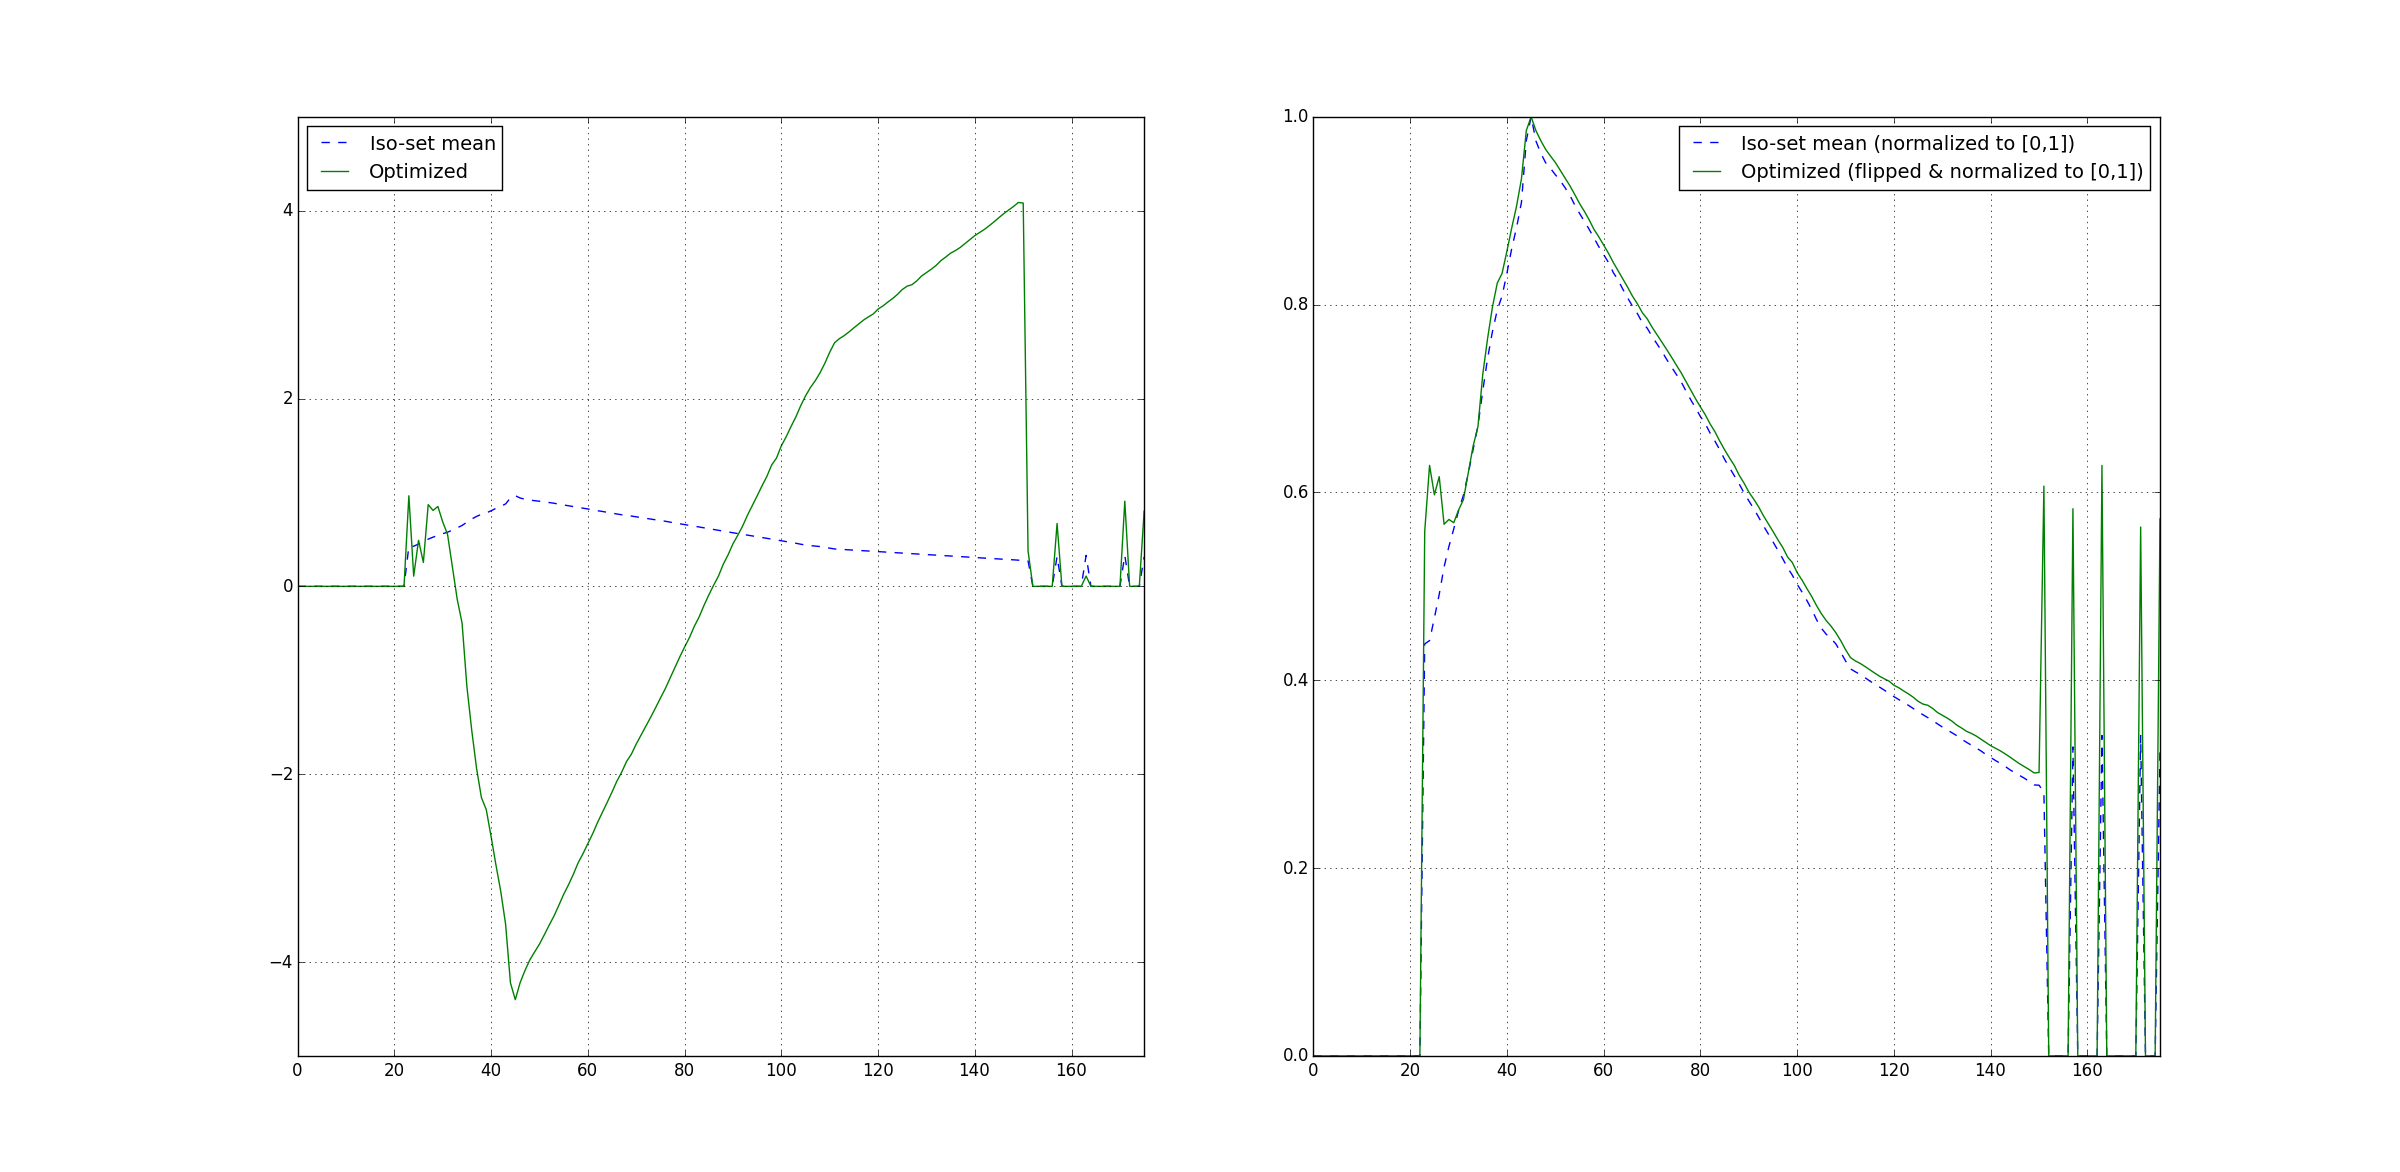
\includegraphics[width=1.0\linewidth]{./images/comparison_optimal_transfers_t1lab.png}}\\
    \subfloat[T1 as a function of T2.]{\label{fig:t2lab_comparison}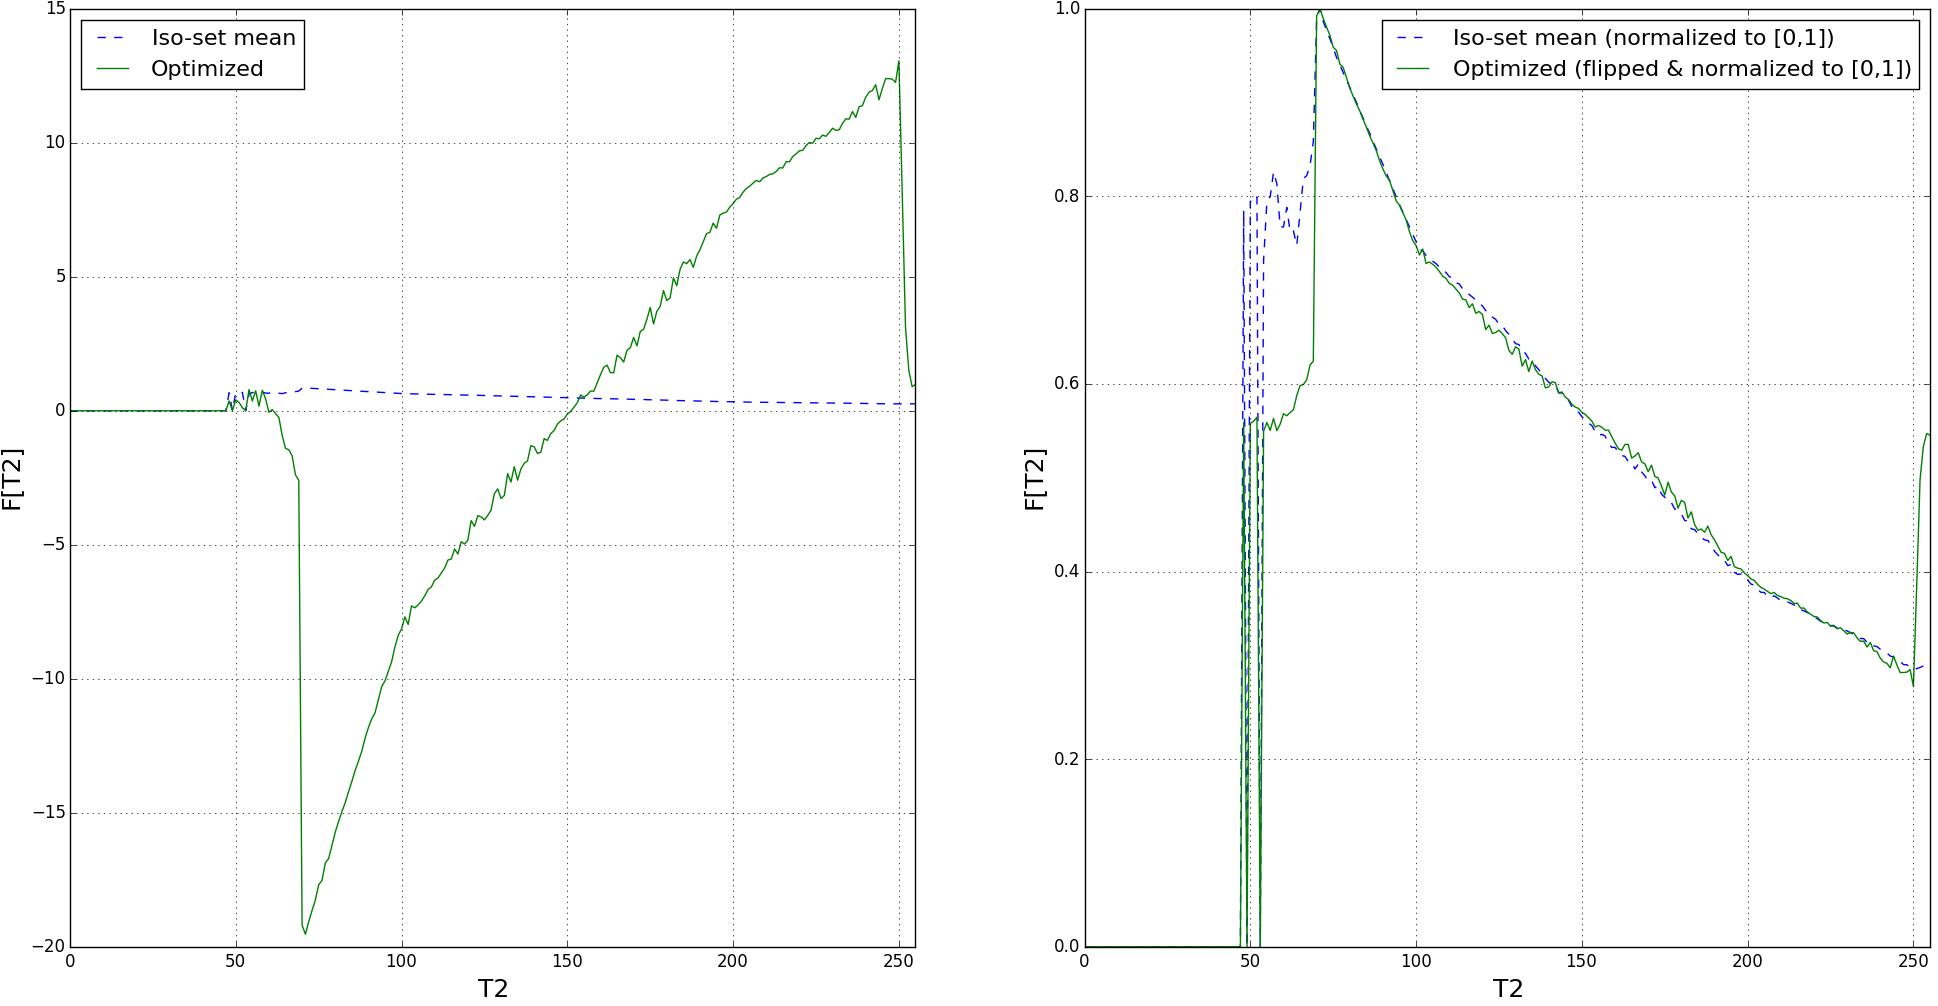
\includegraphics[width=1.0\linewidth]{./images/comparison_optimal_transfers_t2lab.png}}
    \caption{Comparison of optimal transfer functions according to eq. \eqref{eq:ecc_neg_likelihood_vector_form} against the iso-set means (optimal transfer functions used in the Correlation Ratio metric). Input images are shown in figure \ref{fig:brainweb_t1_t2}. The window size was set to radius $4$ voxels ($9\times 9\times 9$). The optimal transfers according to eq. \eqref{eq:ecc_neg_likelihood_vector_form} were obtained using BFGS \citep{GVK502988711}, initializing all elements uniformly at random in [0,1]. Since the vector $\mathbf{f}$ maximizing eq. \eqref{eq:ecc_neg_likelihood_vector_form} is not unique (any affine transform of the optimal $\mathbf{f}$ is optimal too), we may obtain a result very different from the iso-set means (left) but after applying an affine transform normalizing them to $[0,1]$ (normalizing after changing the sign, in this case), the transfer functions are very similar (right).}
\label{fig:comparison_optimal_transfers}
\end{figure}

The effect of introducing the global non-linear transfer into the local linear model is illustrated in fig. \ref{fig:ecc_test_good}. This example is the same as fig. \ref{fig:llr_test}, the fixed image $I$ is the T1, the moving image $J$ is the T2, but instead of fitting the local linear models between $I$ and $J$ directly, we used $F[I]$ and $J$, where $F$ is defined by vector $\mathbf{\bar{f}}$. It can be observed that the non-linear local relationship was made significantly closer to linear by the use of the global transfer function.
\begin{figure*}[t]
\centering
    \subfloat[]{\label{fig:FT1T2_affine_fit_scatter1}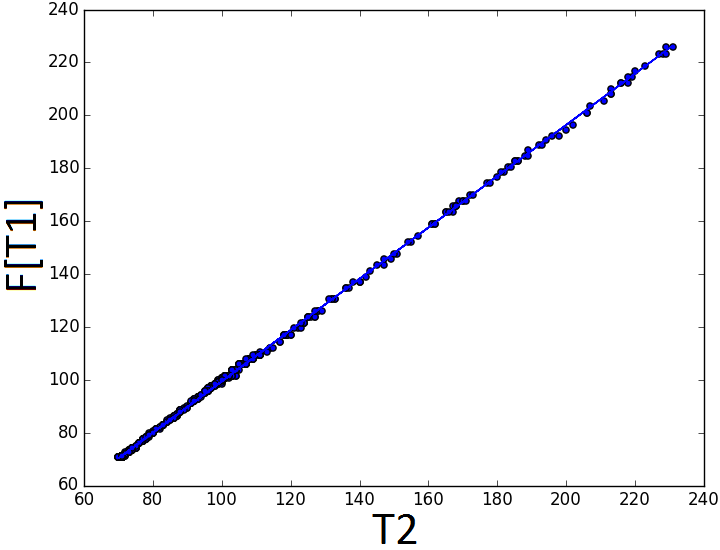
\includegraphics[width=0.2\linewidth]{./images/Ft1_aafo_t2_sample2.png}}
    \subfloat[]{\label{fig:FT1T2_affine_fit_scatter2}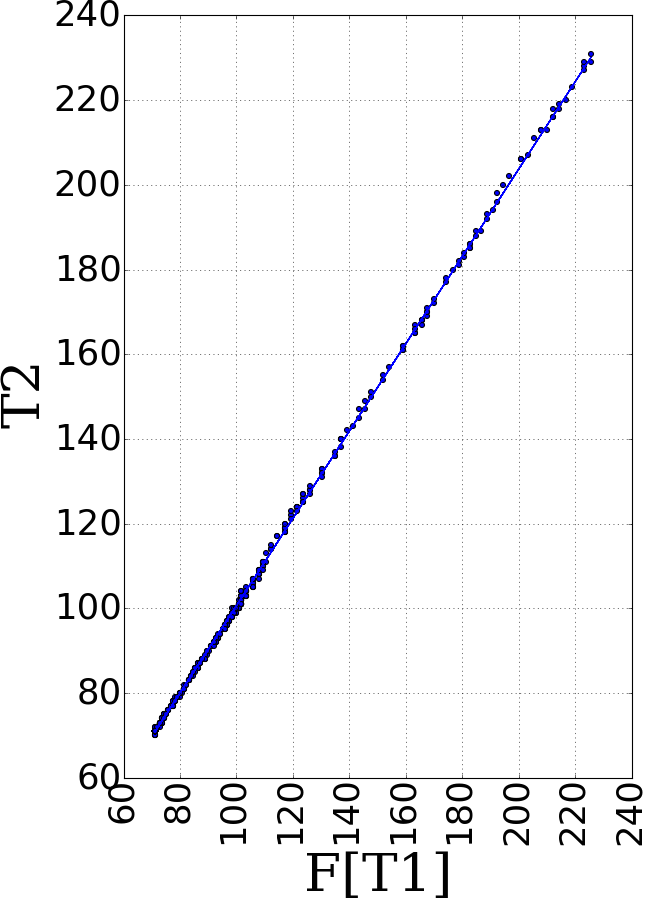
\includegraphics[width=0.2\linewidth]{./images/t2_aafo_Ft1_sample2.png}}
    \subfloat[]{\label{fig:FT1T2_affine_fit_map}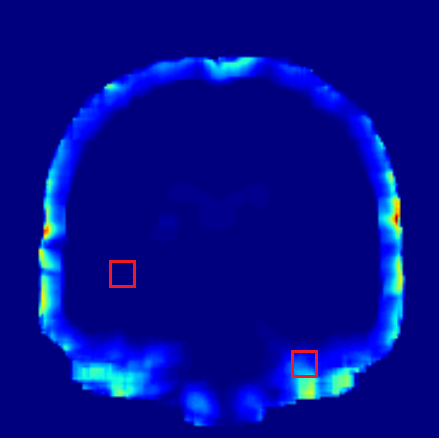
\includegraphics[width=0.2\linewidth]{./images/residuals_t2.png}}
    \subfloat[]{\label{fig:FT1T2_affine_fit_scatter1}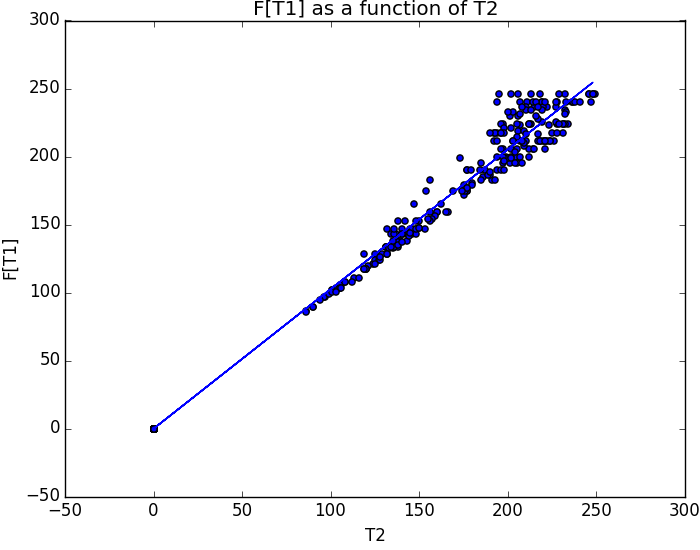
\includegraphics[width=0.2\linewidth]{./images/Ft1_aafo_t2_sample1.png}}
    \subfloat[]{\label{fig:FT1T2_affine_fit_scatter2}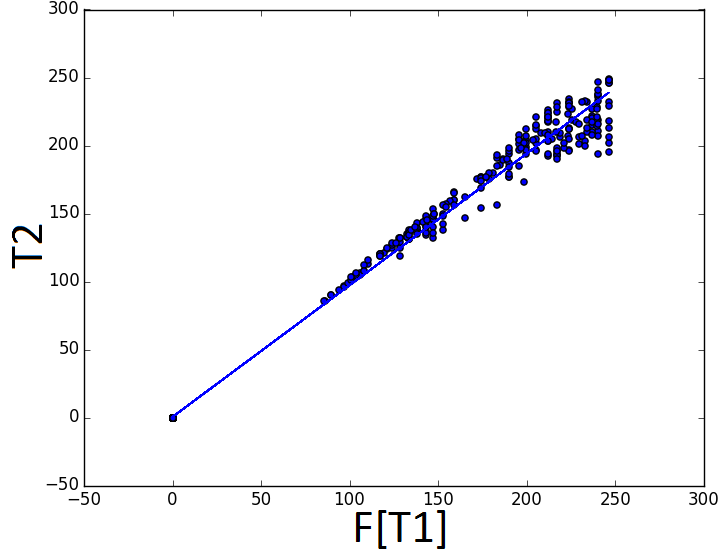
\includegraphics[width=0.2\linewidth]{./images/t2_aafo_Ft1_sample1.png}}\\
    \caption{Local linear reconstruction between T2 intensities and F[T1], where F is the global transfer function used in the Correlation Ratio metric (the average T2 intensity computed over iso-sets of the T1). Center image (c) depicts the reconstruction error in false color (red means high, and blue means low). The selected windows are the same as in figure \ref{fig:llr_test}. The scatter plots depict the best affine fit of F[T1] intensities as a function of T2 (a) and d) ), and the best fit of T2 as a function of F[T1] (b) and e)).}
\label{fig:ecc_test_good}
\end{figure*}
\subsection{Bidirectional transfer functions}

A limitation of existing registration methods that are based on the estimation of a functional relationship between image modalities (such as CR and EM\cite{Roche1998, Roche2000, Arce-santana2014}) is that one of the image modalities must be chosen \emph{a priori} as the target modality (either map intensities from modality A to modality B or viceversa). This is an important decision and what choice is the best may not be obvious in general. To illustrate this, figure \ref{fig:ecc_test_bad} depicts the same example as fig. \ref{fig:ecc_test_good}, but instead of mapping intensities from T1 to T2, we map intensities from T2 to T1. Although the transfer function helps, the relationship is still far from affine. To overcome this limitation, we estimate both transfer functions between $I$ and $J$. Instead of directly computing one single transformation $\phi:\Omega_{I} \rightarrow \Omega_{J}$, we aim to find two invertible transformations (\emph{diffeomorphisms}) $\phi_{I}:\Omega_{I}\rightarrow \Omega_{R}$ and $\phi_{J}:\Omega_{J}\rightarrow \Omega_{R}$ such that the images get aligned in a reference space $\Omega_{R}$ after warping them under $\phi_{I}^{-1}$ and $\phi_{J}^{-1}$ (Fig. \ref{fig:syn_overview}). This is exactly the same formulation as the SyN algorithm proposed by Avants {\it et al.} \cite{Avants2011}, and explained in section \ref{sec:non_linear_image_registration}, where the partial transforms $\phi_{I}, \phi_{J}$ are the middle-point diffeomorphisms of a diffeomorphic flow transforming the domains $\Omega_{I}, \Omega_{J}$ toward each other.\\

\begin{figure*}[t]
\centering
    \subfloat[]{\label{fig:T1FT2_affine_fit_scatter1}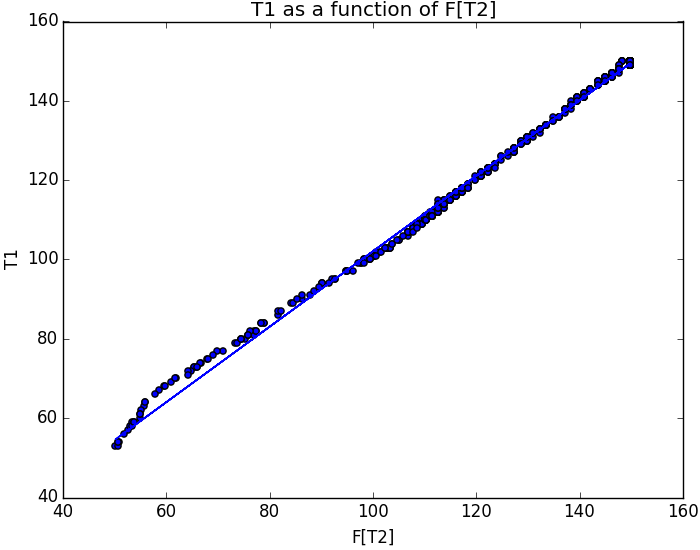
\includegraphics[width=0.2\linewidth]{./images/t1_aafo_Ft2_sample2.png}}
    \subfloat[]{\label{fig:T1FT2_affine_fit_scatter2}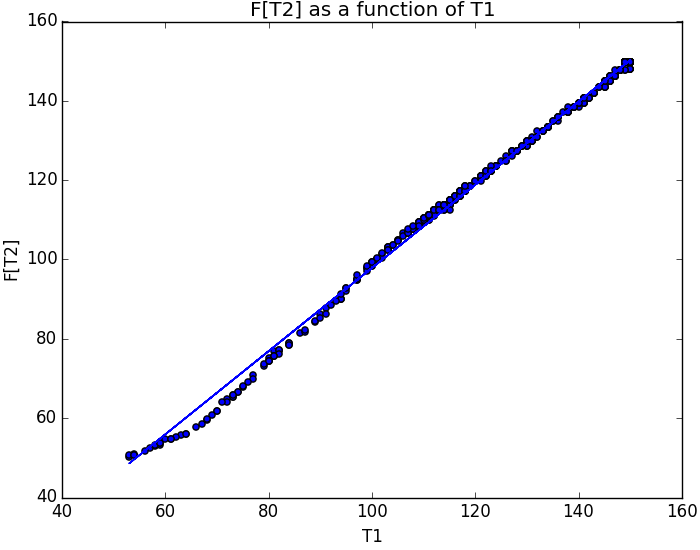
\includegraphics[width=0.2\linewidth]{./images/Ft2_aafo_t1_sample2.png}}
    \subfloat[]{\label{fig:T1FT2_affine_fit_map}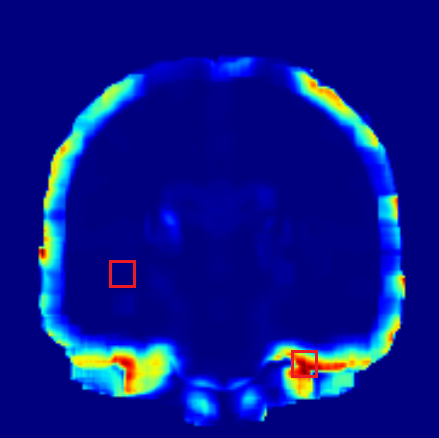
\includegraphics[width=0.2\linewidth]{./images/residuals_t1.png}}
    \subfloat[]{\label{fig:T1FT2_affine_fit_scatter1}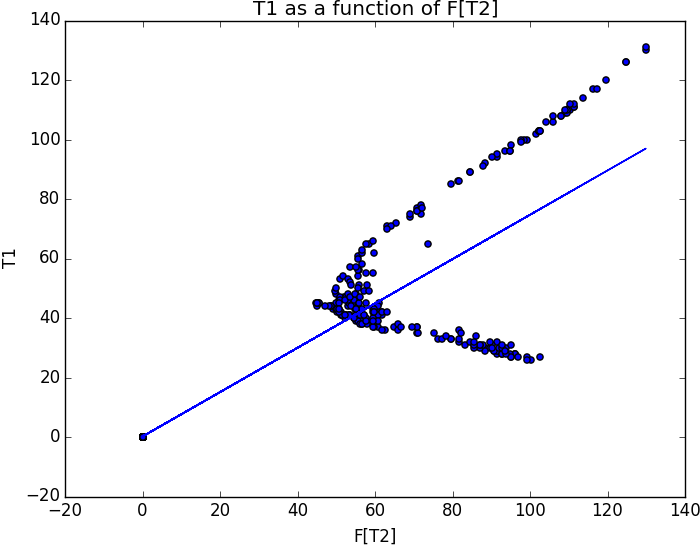
\includegraphics[width=0.2\linewidth]{./images/t1_aafo_Ft2_sample1.png}}
    \subfloat[]{\label{fig:T1FT2_affine_fit_scatter2}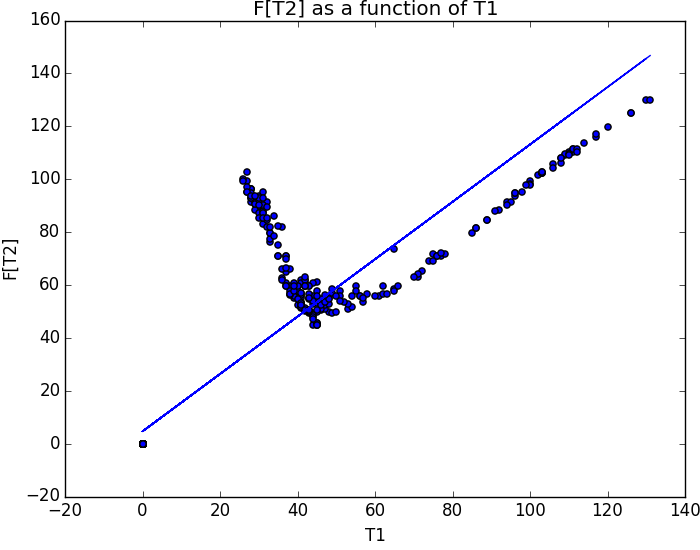
\includegraphics[width=0.2\linewidth]{./images/Ft2_aafo_t1_sample1.png}}\\
    \caption{.}
\label{fig:ecc_test_bad}
\end{figure*}

\begin{figure}[t]
\centering
\fbox{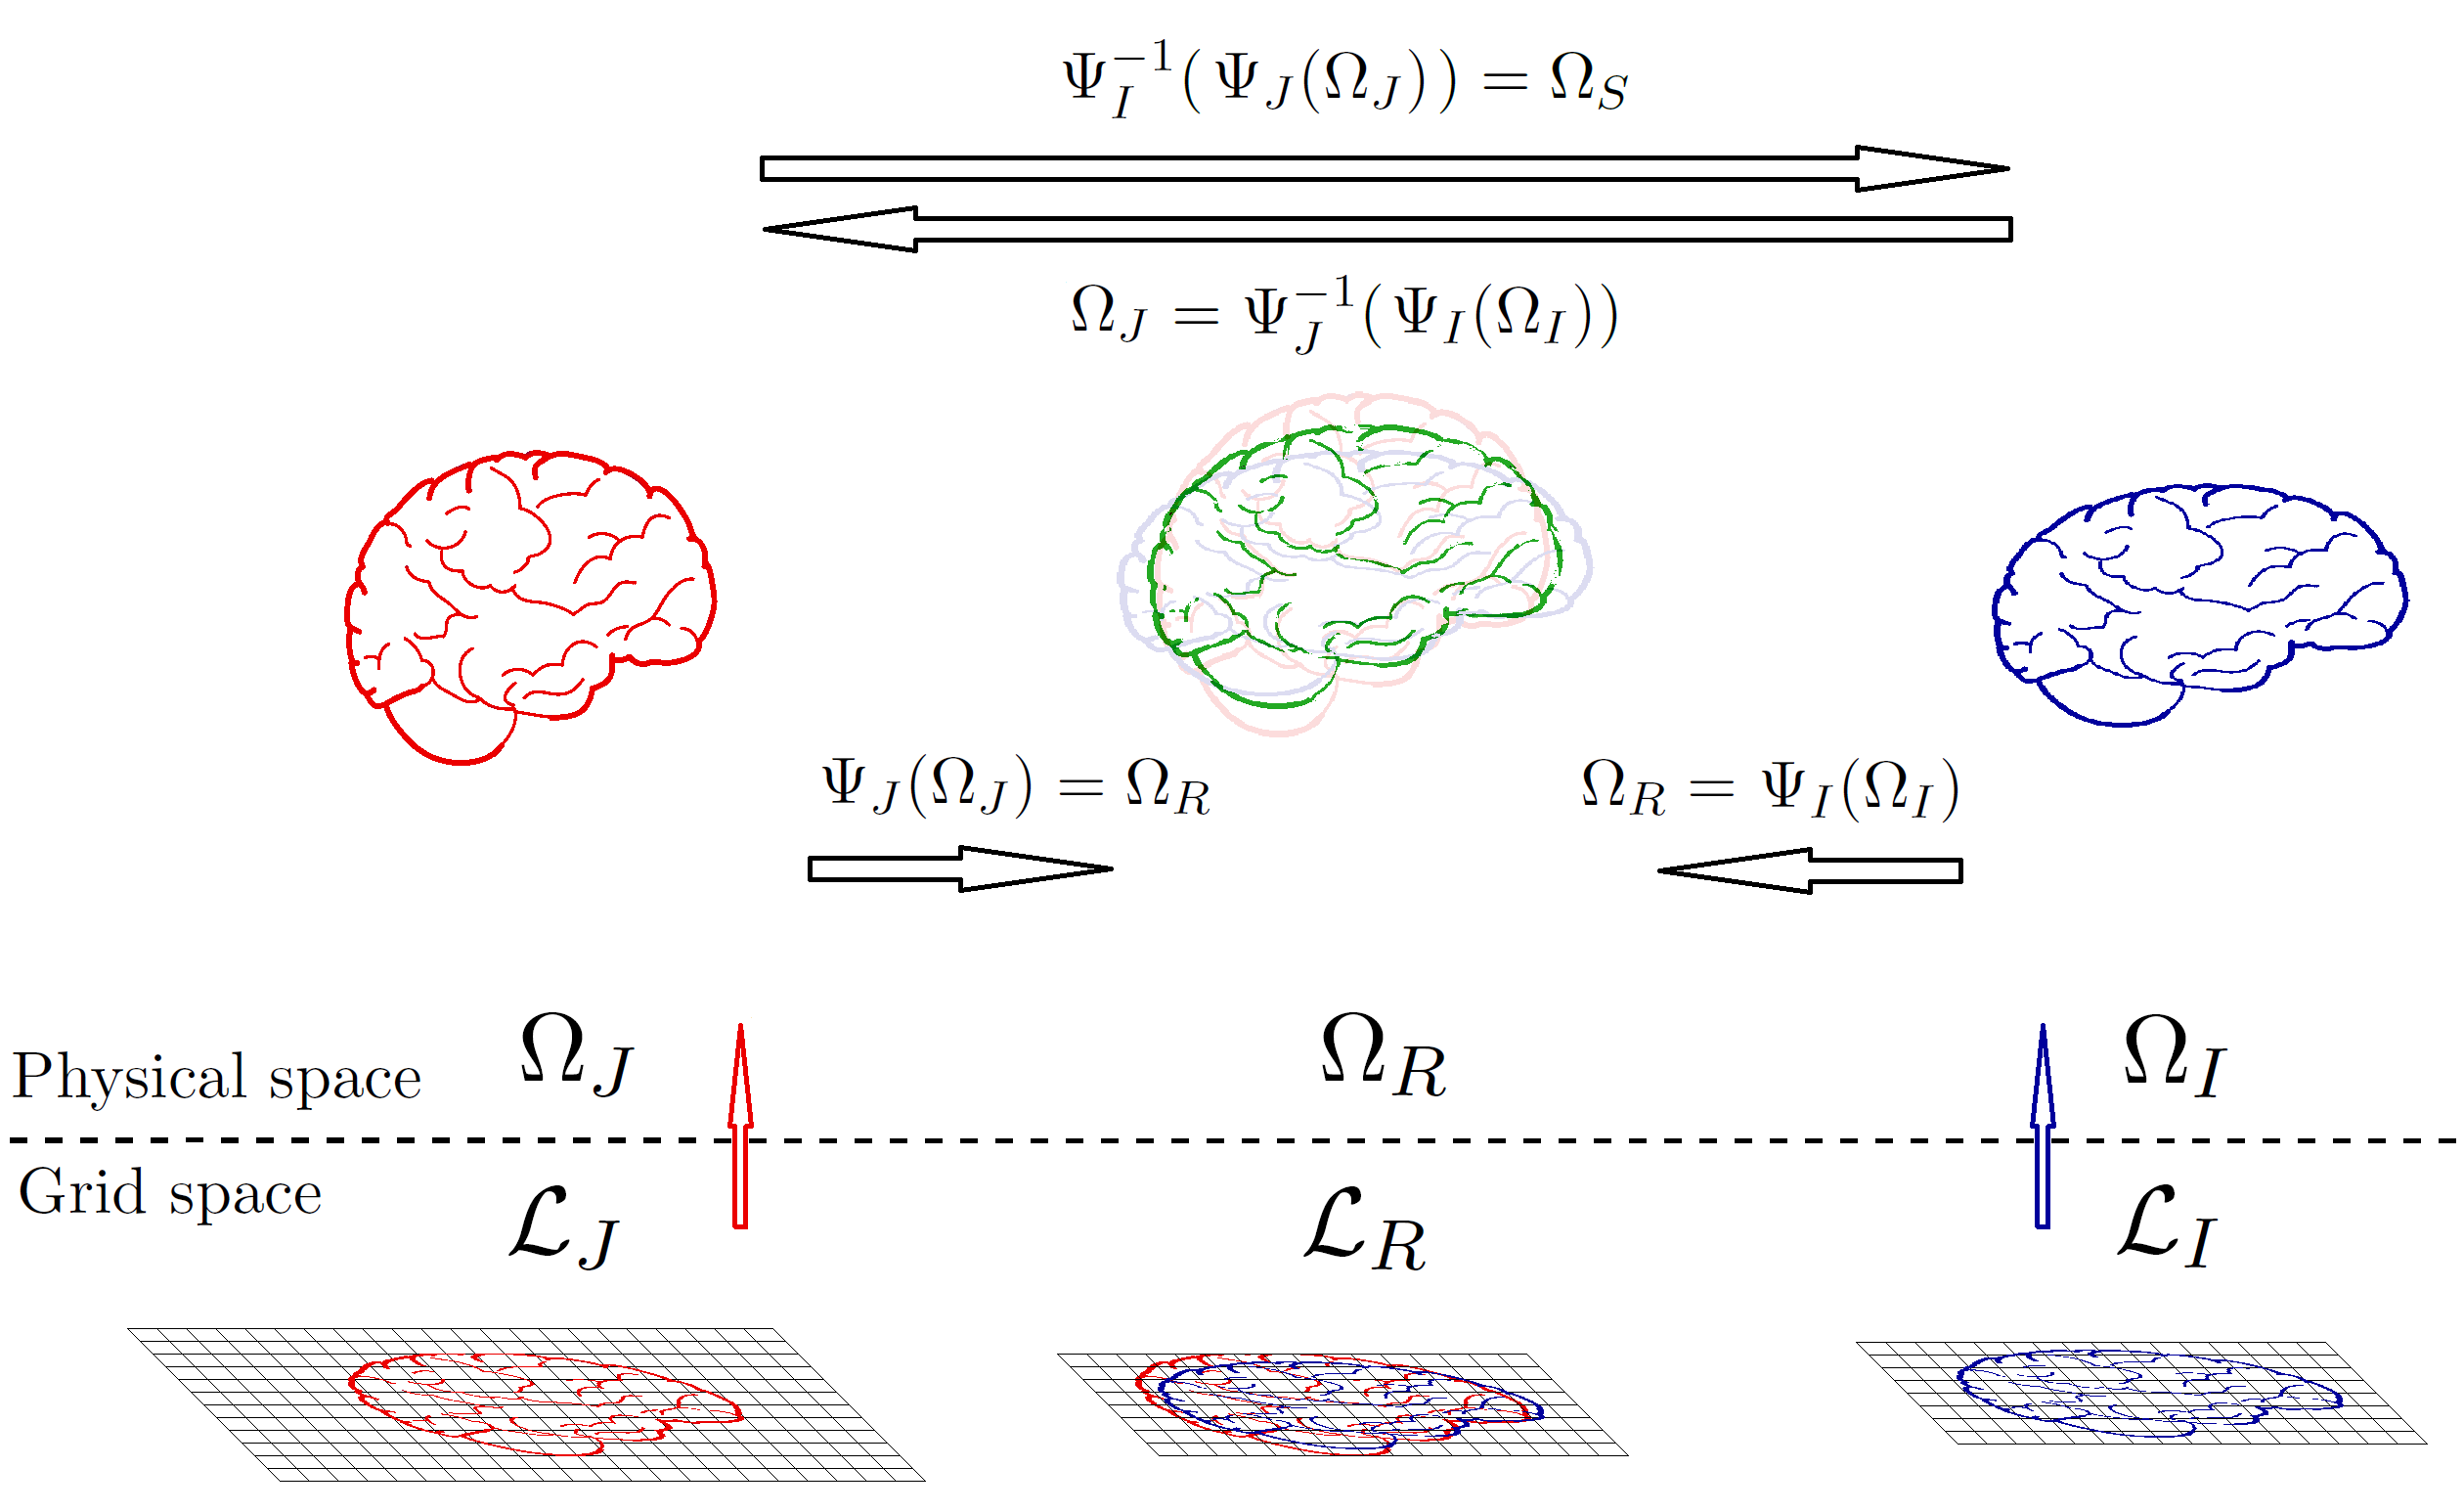
\includegraphics[width=1.0\linewidth]{./images/syn_overview.png}}
\caption{The Greedy SyN algorithm registers two input images by computing two diffeomorphisms that map the input images towards a common reference domain. The final
diffeomorphism is computed by composing the two partial diffeomorphisms.}
\label{fig:syn_overview}
\end{figure}

Our model (eq. \eqref{eq:ecc_model}) may be symmetrized by introducing both transfer functions between image modalities and considering both transformations according to the SyN transformation model as follows. As before, consider a rectangular local window $W_{v}$ but this time centered at a voxel $v$ in the reference space $v\in\Omega_{R}$. Denote by
\begin{align*}
    \mathbf{x}_{v}' &= \left(I(\phi_{I}^{-1}(v_{1})), I(\phi_{I}^{-1}(v_{2})), ..., I(\phi_{I}^{-1}(v_{n}))\right)^{T}\\
    \mathbf{y}_{v}' &= \left(J(\phi_{J}^{-1}(v_{1})), J(\phi_{J}^{-1}(v_{2})), ..., J(\phi_{J}^{-1}(v_{n}))\right)^{T},
\end{align*}
the (non-centered) images $I, J$ evaluated at all voxels of the local window $v_{i}\in W_{v}, i=1, 2, .., n$, and let $\mathbf{x}_{v} = \mathbf{x}_{v}' - \frac{\mathbf{x}_{v}^{T}\mathbbm{1}}{n}$, and $\mathbf{y}_{v} = \mathbf{y}_{v}' - \frac{\mathbf{y}_{v}^{T}\mathbbm{1}}{n}$ be their centered counterparts. Note that this time, both vectors $\mathbf{x}_{v}$ and $\mathbf{y}_{v}$ are moving according to the (inverses of the) transforms $\phi_{I}$ and $\phi_{J}$. By introducing both transfer functions, $F_{I}$ and $F_{J}$ mapping intensities from $I$ to $J$ and from $J$ to $I$ respectively, our symmetric model may be written as follows:
\begin{equation}\label{eq:symmetric_ecc_model}
    \begin{array}{ccccc}
        \frac{\mathbf{y}_{v}}{||\mathbf{y}_{v}||} = \left[F_{I}\left[\mathbf{x}_{v}\right] \; \mathbbm{1}\right]\alpha + \eta_{I}(v) \; \forall v\in\Omega_{R}\\
        \frac{\mathbf{x}_{v}}{||\mathbf{x}_{v}||} = \left[F_{J}\left[\mathbf{y}_{v}\right] \; \mathbbm{1}\right]\beta + \eta_{J}(v) \; \forall v\in\Omega_{R}\\
    \end{array}.
\end{equation}
By assuming independence between the two sets of normally distributed random vectors $\eta_{I}$ and $\eta_{I}$, it follows immediately that maximizing the log-likelihood of model \eqref{eq:symmetric_ecc_model} is equivalent to maximizing the (symmetric) ECC matching functional:
\begin{equation*}
    ECC(I, J;\phi_{I}, \phi_{J}) = CC(\mathbbm{E}[J|I], J ; \phi_{J}) + CC(\mathbbm{E}[I|J], I ; \phi_{I})
\end{equation*}
%the negative log likelyhood is proportional to
%\begin{displaymath}
%    U(I, J;\phi) =
%    \sum_{v\in\Omega_{R}}\left(1-\frac{\left(F_{I}\left[\mathbf{x}_{v}\right]^{T} \mathbf{y}_{v}\right)^{2}}{||F_{I}\left[\mathbf{x}_{v}\right]||^{2}||\mathbf{y}_{v}||^{2}}\right) %+
%    \left(1-\frac{\left(F_{J}\left[\mathbf{y}_{v}\right]^{T} \mathbf{x}_{v}\right)^{2}}{||F_{J}\left[\mathbf{y}_{v}\right]||^{2}||\mathbf{x}_{v}||^{2}}\right),
%\end{displaymath}
%and the maximum likelihood estimator for $\phi_{I}$ and $\phi_{J}$ can be obtain by maximizing the symmetric Expected Cross Correlation:
%\begin{equation}
%    ECC(I, J;\phi) =
%    \sum_{v\in\Omega_{R}}\frac{\left(F_{I}\left[\mathbf{x}_{v}\right]^{T} \mathbf{y}_{v}\right)^{2}}{||F_{I}\left[\mathbf{x}_{v}\right]||^{2}||\mathbf{y}_{v}||^{2}} +
%    \frac{\left(F_{J}\left[\mathbf{y}_{v}\right]^{T} \mathbf{x}_{v}\right)^{2}}{||F_{J}\left[\mathbf{y}_{v}\right]||^{2}||\mathbf{x}_{v}||^{2}}
%\end{equation}



\iffalse
\begin{figure}[t!]
    \subfloat[]{\label{fig:epicor_b0up_ecc.png}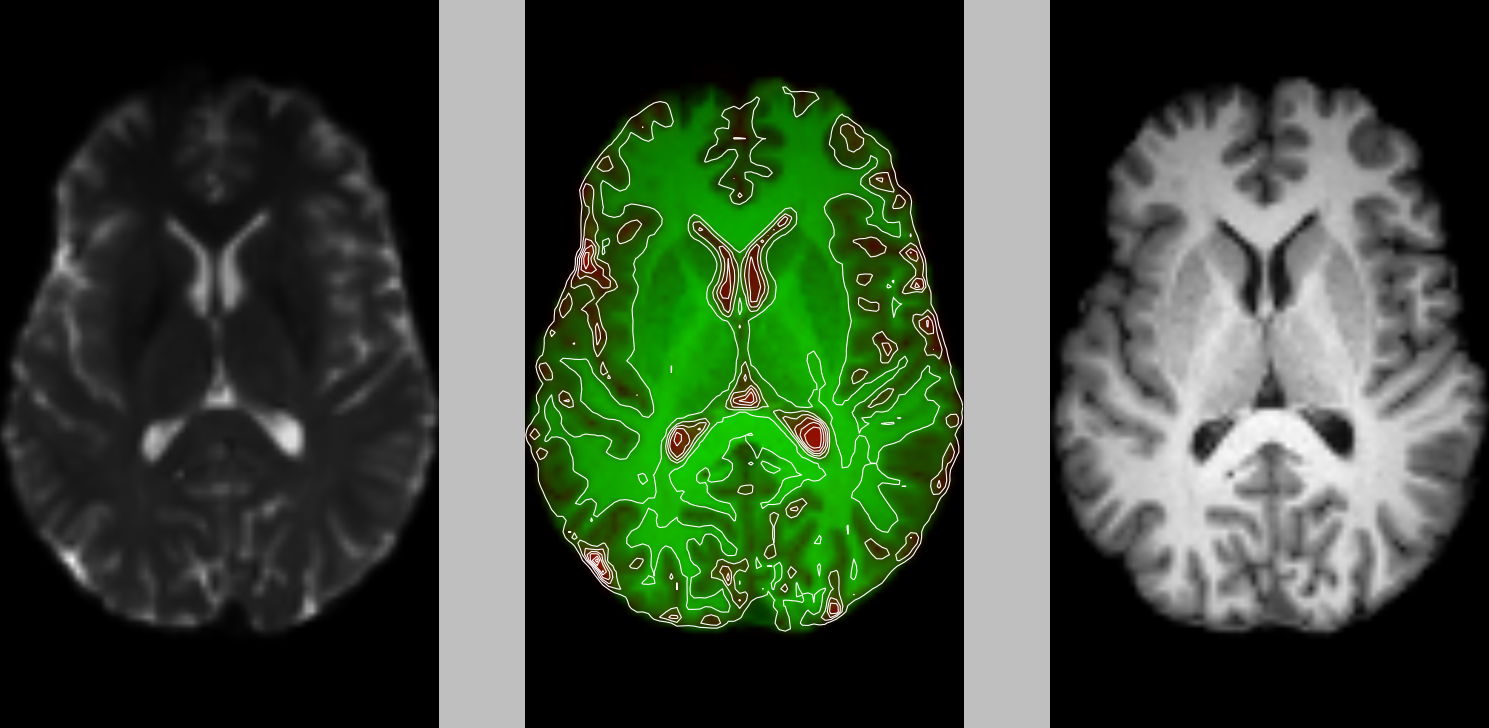
\includegraphics[width=1\linewidth]{./images/T1B0Result/epicor_b0up_ecc.png}}\\
    \subfloat[]{\label{fig:epicor_b0up_mi.png}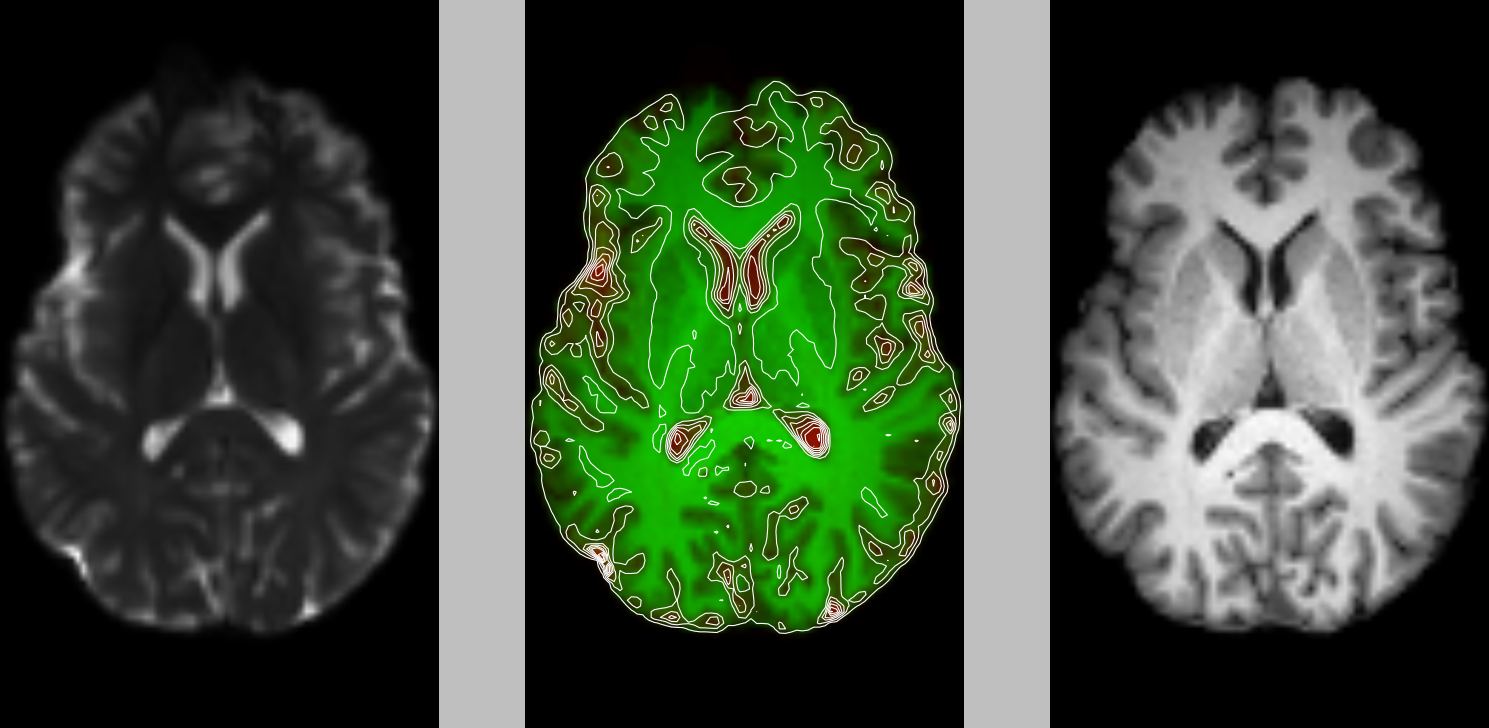
\includegraphics[width=1\linewidth]{./images/T1B0Result/epicor_b0up_mi.png}}\\
    \caption{Registration of B0(blip up) to T1.}
\label{fig:epicor_up_ecc}
\end{figure}

\begin{figure}[t!]
\centering
    \subfloat[]{\label{fig:b0_up_sagital_zoom}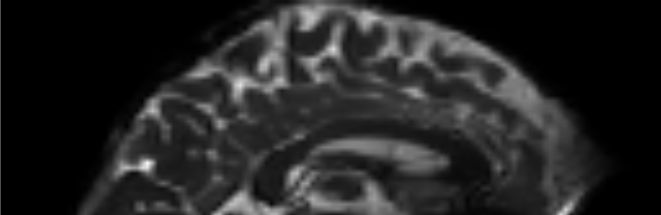
\includegraphics[width=0.5\linewidth]{./images/T1B0Result/b0_up_sagital_zoom.png}}
    \subfloat[]{\label{fig:affine_mi_t1b0up_sagital_zoom.png}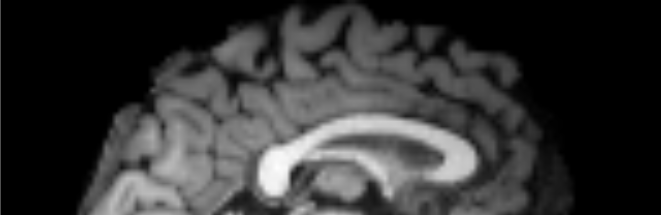
\includegraphics[width=0.5\linewidth]{./images/T1B0Result/affine_mi_t1b0up_sagital_zoom.png}}\\
    \subfloat[]{\label{fig:synecc_contours_t1b0up_sagital_zoom}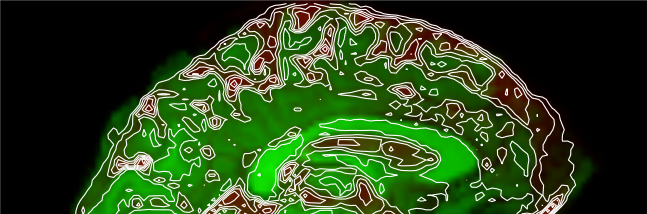
\includegraphics[width=0.5\linewidth]{./images/T1B0Result/synecc_contours_t1b0up_sagital_zoom.png}}
    \subfloat[]{\label{fig:synmi_contours_t1b0up_sagital_zoom}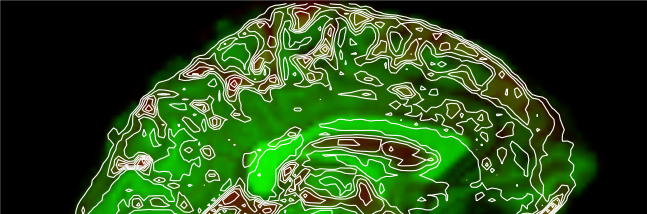
\includegraphics[width=0.5\linewidth]{./images/T1B0Result/synmi_contours_t1b0up_sagital_zoom.png}}\\
    \subfloat[]{\label{fig:synecc_t1b0up_sagital_zoom}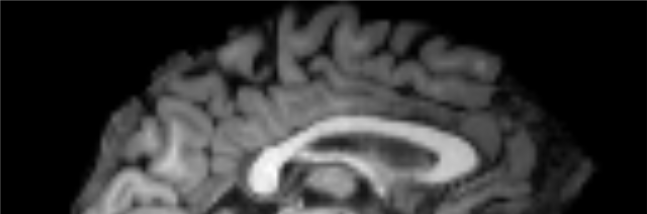
\includegraphics[width=0.5\linewidth]{./images/T1B0Result/synecc_t1b0up_sagital_zoom.png}}
    \subfloat[]{\label{fig:synmi_t1b0up_sagital_zoom}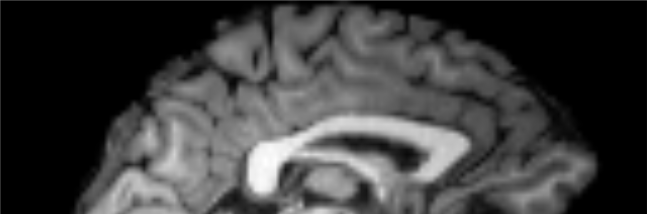
\includegraphics[width=0.5\linewidth]{./images/T1B0Result/synmi_t1b0up_sagital_zoom.png}}\\
    \caption{Registration of T1 to B0(blip up).}
\label{fig:sagital_zoom_t1b0up}
\end{figure}


\begin{figure}[t!]
    \subfloat[]{\label{fig:epicor_b0down_ecc.png}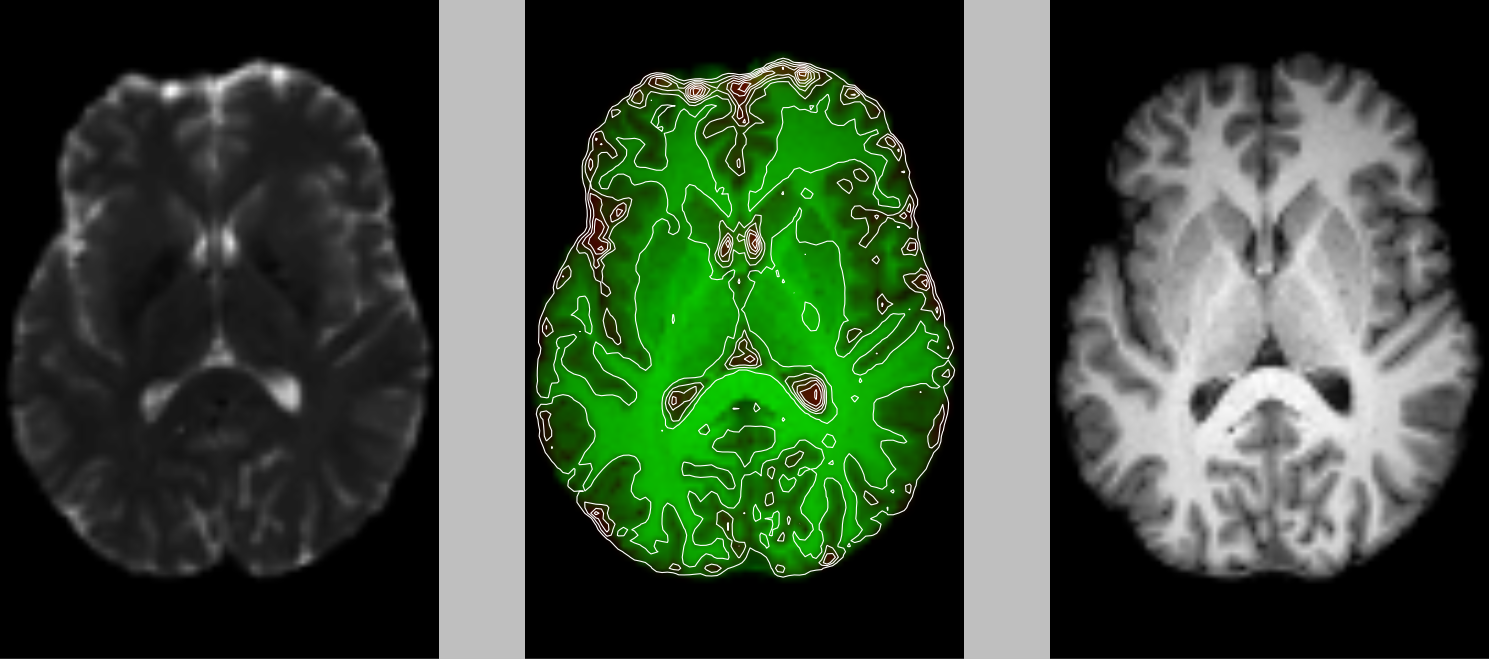
\includegraphics[width=1\linewidth]{./images/T1B0Result/epicor_b0down_ecc.png}}\\
    \subfloat[]{\label{fig:epicor_b0down_mi.png}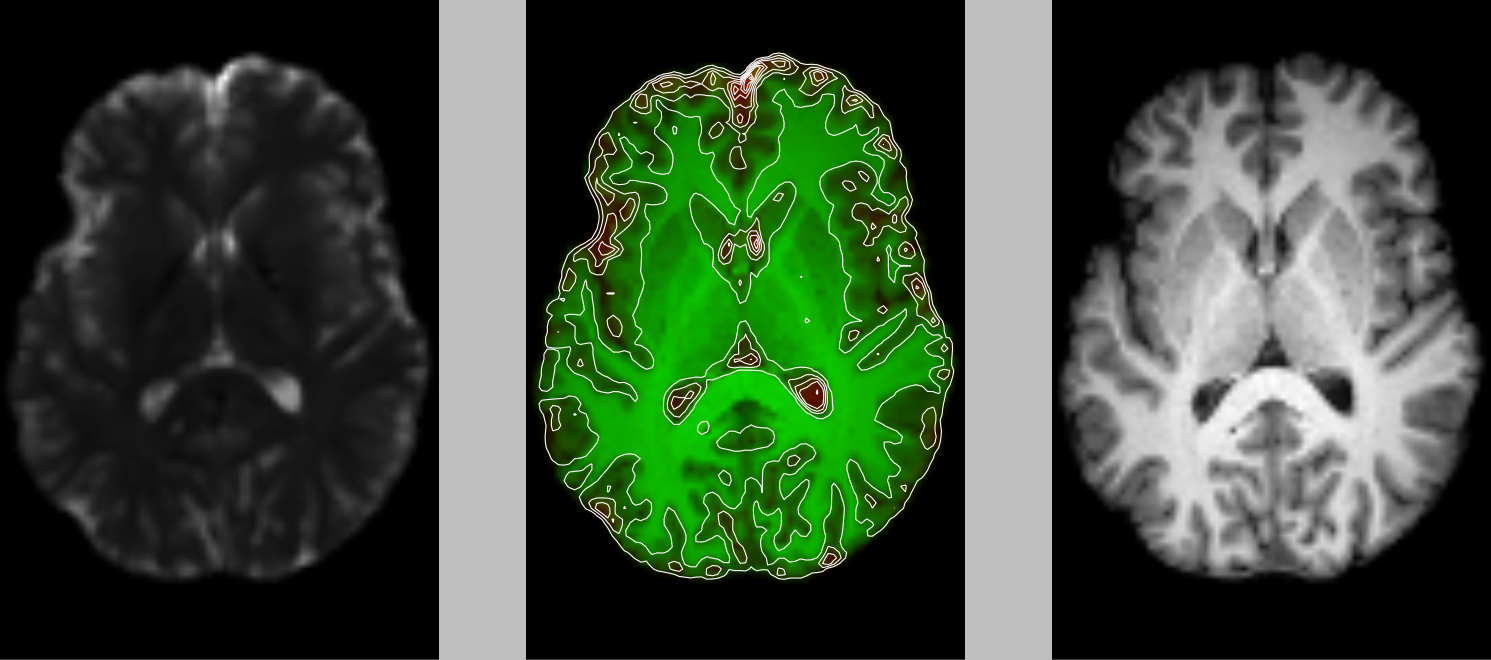
\includegraphics[width=1\linewidth]{./images/T1B0Result/epicor_b0down_mi.png}}\\
    \caption{Registration of B0(blip up) to T1.}
\label{fig:epicor_down_ecc}
\end{figure}

\begin{figure}[t!]
\centering
    \subfloat[]{\label{fig:b0_down_sagital_zoom}
\includegraphics[width=0.5\linewidth]{./images/T1B0Result/b0_down_sagital_zoom.png}}
    \subfloat[]{\label{fig:t1_sagital_zoom}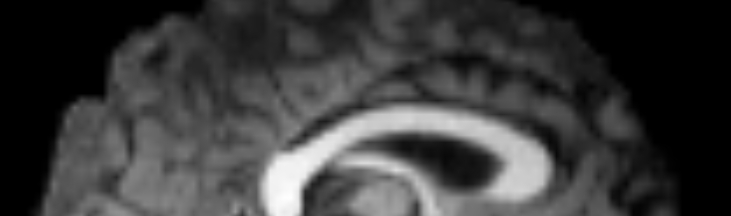
\includegraphics[width=0.5\linewidth]{./images/T1B0Result/t1_sagital_zoom.png}}\\
    \subfloat[]{\label{fig:synecc_contours_t1b0_sagital_zoom}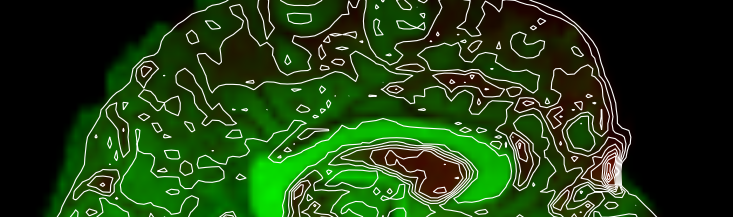
\includegraphics[width=0.5\linewidth]{./images/T1B0Result/synecc_contours_t1b0_sagital_zoom.png}}
    \subfloat[]{\label{fig:synmi_contours_t1b0_sagital_zoom}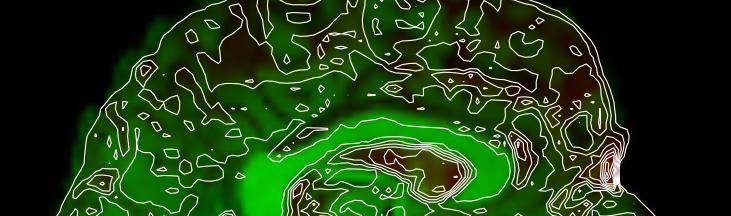
\includegraphics[width=0.5\linewidth]{./images/T1B0Result/synmi_contours_t1b0_sagital_zoom.png}}\\
    \subfloat[]{\label{fig:synecc_t1b0_sagital_zoom}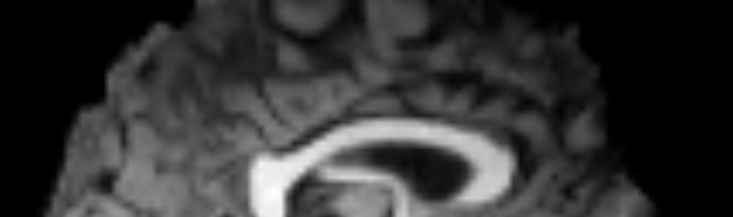
\includegraphics[width=0.5\linewidth]{./images/T1B0Result/synecc_t1b0_sagital_zoom.png}}
    \subfloat[]{\label{fig:synmi_t1b0_sagital_zoom}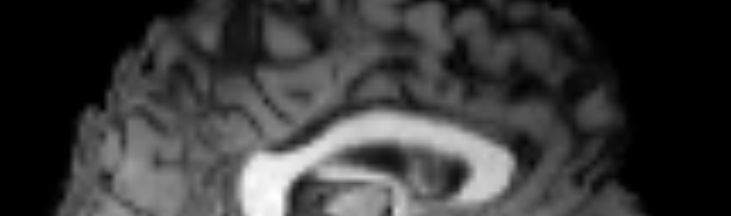
\includegraphics[width=0.5\linewidth]{./images/T1B0Result/synmi_t1b0_sagital_zoom.png}}\\
    \caption{Registration of T1 to B0(blip down).}
\label{fig:sagital_zoom_t1b0down}
\end{figure}


\begin{figure}[t!]
    \subfloat[]{\label{fig:jaccard_T1_B0}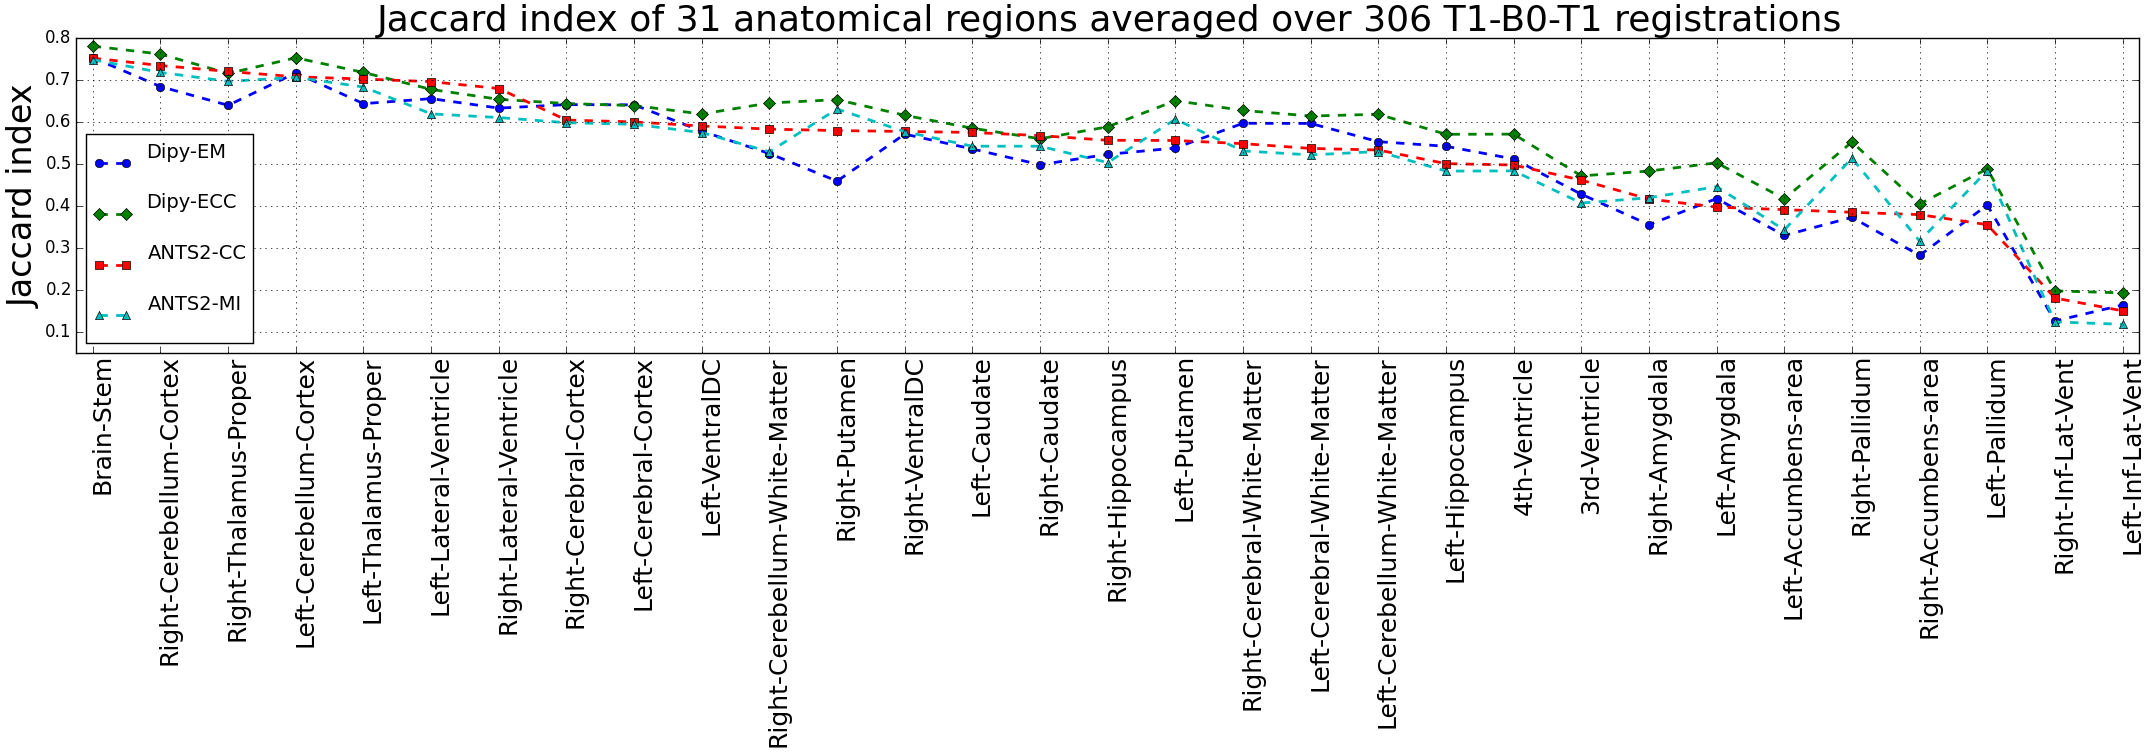
\includegraphics[width=1\linewidth]{./images/T1B0Result/jaccard_T1_B0.png}}\\
    \subfloat[]{\label{fig:jaccard_boxplots_T1_B0}\includegraphics[width=1\linewidth]{./images/T1B0Result/jaccard_boxplots_T1_B0.png}}\\
    \caption{Registration result of B0(blip down) to T1.}
\label{fig:epicor_down_ecc}
\end{figure}

\fi 
\section{Experiments}
We compared the accuracy of four matching functionals driving the SyN transformation model: CC, MI, EM and ECC. We selected the CC functional because its robustness and accuracy for mono-modal registration have been demonstrated in large scale comparative studies \citep{Klein2009, Klein2010, Rohlfing2012} (it would be desirable to reach similar performance in the multi-modal case), we would like to quantify how large is its drop in accuracy for multi-modal images. MI \citep{Maes1997, Mattes2003} may be considered the functional of choice for multi-modal registration, it is expected that any new developed functional yields results at least as good as MI. The EM functional \cite{Arce-santana2014} is, to the best of our knowledge, the most recent proposal for multi-modal registration based on the assumption of a functional relationship between image modalities. It introduces a measure of uncertainty for each intensity, which may help to alleviate the effects of non-stationary relationships between image intensities. We implemented the EM functional to drive the SyN transformation model and extended it to make it symmetric (to estimate both transfer functions instead of only one), in our experiments, these modifications performed significantly better than the basic functional (non-symmetric, and using an elastic transformation model) proposed by Arce {\it et al.}\cite{Arce-santana2014}. Both MI and EM are voxel-wise functionals (i.e. it compares pairs of single voxels), while CC and ECC are computed from local rectangular windows.

\subsection{Mono-modal registration}
Although our matching functional was designed for multi-modal image registration, it is important to first verify that the quality of the algorithms is reasonable for mono-modal registration. Figure \ref{fig:mono_graph_seg} show the average overlap score for each of 31 manually annotated anatomical regions from the IBSR database. Note that the Jaccard indices obtained with CC (i.e. ANTS) are higher than reported by Rohlfing \cite{Rohlfing2012}. In his experiments, he used three resolutions with a maximum of 10, 10 and 5 iterations only. Here, we set a maximum of 100, 100 and 25 iterations, leaving the rest of the parameters unchanged (the same for all functionals). We can see that SyN with the EM metric is very competitive, but still not as good as CC. This may be explained by the fact that CC uses a window centered at each voxel for computing the similarity, while the EM is voxelwise. This behavior can also be observed from the results of SyN with Mutual Information (MI), which is also voxel-wise and very competitve but not as good as CC. By considering neighborhoods of the same size, the performance of ECC is practically the same as CC. Table \ref{tab:monomodal_results_segTri_fill} shows the overlap scores over tissue types (white matter, gray matter and cerebrospinal fluid), instead of anatomical areas.
%Table \ref{tab:monomodal_results_seg} and
%% Table generated by Excel2LaTeX from sheet 'SyNEM-Monomodal-Large'
\begin{table}[p]
\begin{adjustwidth}{-0.75cm}{}
  {\centering
    \small
    \begin{tabular}{lcccc}
    \toprule
    \textbf{}& \textbf{SyN-EM} & \textbf{SyN-ECC} & \textbf{SyN-CC} & \textbf{SyN-MI} \\
    \midrule
    \textbf{Brain-Stem} & 0.786 & \textbf{0.816} & 0.812 & 0.804 \\
    \textbf{Right-Cerebellum-Cortex} & 0.736 & \textbf{0.815} & 0.813 & 0.771 \\
    \textbf{Left-Cerebellum-Cortex} & 0.739 & \textbf{0.811} & 0.808 & 0.766 \\
    \textbf{Right-Thalamus-Proper} & 0.714 & 0.766 & \textbf{0.772} & 0.745 \\
    \textbf{Left-Thalamus-Proper} & 0.727 & 0.763 & \textbf{0.767} & 0.748 \\
    \textbf{Right-Putamen} & 0.681 & 0.748 & \textbf{0.751} & 0.712 \\
    \textbf{Left-Putamen} & 0.699 & 0.744 & \textbf{0.744} & 0.721 \\
    \textbf{Left-Cerebral-Cortex} & 0.724 & \textbf{0.739} & 0.733 & 0.687 \\
    \textbf{Right-Cerebral-Cortex} & 0.719 & \textbf{0.739} & 0.731 & 0.683 \\
    \textbf{Right-Cerebral-White-Matter} & 0.702 & \textbf{0.733} & 0.720 & 0.645 \\
    \textbf{Left-Cerebral-White-Matter} & 0.705 & \textbf{0.732} & 0.721 & 0.646 \\
    \textbf{Left-Lateral-Ventricle} & 0.731 & 0.727 & \textbf{0.732} & 0.718 \\
    \textbf{Right-Lateral-Ventricle} & 0.709 & 0.714 & \textbf{0.717} & 0.699 \\
    \textbf{Right-Cerebellum-White-Matter} & 0.576 & \textbf{0.701} & 0.691 & 0.608 \\
    \textbf{Left-Cerebellum-White-Matter} & 0.581 & \textbf{0.701} & 0.693 & 0.611 \\
    \textbf{Left-Caudate} & 0.645 & \textbf{0.671} & 0.665 & 0.666 \\
    \textbf{Right-Caudate} & 0.620 & \textbf{0.655} & 0.647 & 0.651 \\
    \textbf{Right-VentralDC} & 0.612 & 0.651 & \textbf{0.652} & 0.628 \\
    \textbf{Left-VentralDC} & 0.622 & \textbf{0.651} & 0.650 & 0.631 \\
    \textbf{Right-Pallidum} & 0.498 & \textbf{0.622} & 0.620 & 0.582 \\
    \textbf{Right-Hippocampus} & 0.572 & \textbf{0.621} & 0.620 & 0.575 \\
    \textbf{Left-Pallidum} & 0.524 & \textbf{0.615} & 0.614 & 0.583 \\
    \textbf{Left-Hippocampus} & 0.574 & \textbf{0.610} & 0.609 & 0.564 \\
    \textbf{4th-Ventricle} & 0.551 & 0.606 & \textbf{0.608} & 0.574 \\
    \textbf{3rd-Ventricle} & 0.527 & 0.544 & \textbf{0.547} & 0.515 \\
    \textbf{Left-Amygdala} & 0.444 & 0.519 & \textbf{0.519} & 0.484 \\
    \textbf{Right-Amygdala} & 0.411 & 0.513 & \textbf{0.514} & 0.458 \\
    \textbf{Left-Accumbens-area} & 0.451 & 0.500 & \textbf{0.500} & 0.462 \\
    \textbf{Right-Accumbens-area} & 0.433 & 0.490 & \textbf{0.490} & 0.443 \\
    \textbf{Right-Inf-Lat-Vent} & 0.177 & 0.230 & \textbf{0.232} & 0.162 \\
    \textbf{Left-Inf-Lat-Vent} & 0.190 & 0.228 & \textbf{0.233} & 0.167 \\
    \hline
    \textbf{Average (std.)} & 0.593 (0.148) & 0.644 (0.142) & 0.643 (0.140) & 0.603 (0.149) \\
    \textbf{Rank-1 count} & 0 & 16 & 15 & 0 \\
    \textbf{Rank-2 count} & 1 & 14 & 14 & 2 \\
    \textbf{Rank-3 count} & 9 & 1 & 2 & 19 \\
    \bottomrule
    \end{tabular}}%
    \caption{Comparison of the registration performance (measured by the Jaccard index over 31 anatomical regions) of the Greedy SyN algorithm with EM, ECC, CC and MI metrics.
The Jaccard indices were averaged over 306 monomodal registrations. Rank-$k$ counts show the number of anatomical regions for which each
method ranked $k$ among the four methods under comparison. Top performer (rank-1) for each region is highlighted. }
  \label{tab:monomodal_results_seg}%
\end{adjustwidth}
\end{table}%

% Table generated by Excel2LaTeX from sheet 'SyNEM-Monomodal-Large'
\begin{table}[htbp]
  \centering
  {\small
    \begin{tabular}{rrrr}
    \toprule
    \textbf{} & \textbf{SyN-EM} & \textbf{SyN-ECC} & \textbf{SyN-CC} \\
    \midrule
    \textbf{Background} & 0.994 & 0.995 & \textbf{0.995} \\
    \textbf{CSF} & 0.335 & 0.349 & \textbf{0.359} \\
    \textbf{Gray Matter} & 0.740 & \textbf{0.765} & 0.759 \\
    \textbf{White Matter} & 0.703 & \textbf{0.739} & 0.728 \\
    \bottomrule
    \end{tabular}%
    \caption{Comparison of the registration performance (measured by the Jaccard index over Background, CSF, GM and WM)of the Greedy SyN algorithm with EM, ECC and CC metrics. The Jaccard
indices were averaged over 306 monomodal registrations. Top performer for each region is highlighted.}
  \label{tab:monomodal_results_segTri_fill}}%
\end{table}%


\begin{figure*}[t!]
\centering
\includegraphics[width=1.0\linewidth]{./images/mono_lines_seg.png}\\
\caption{{\small Comparison of the registration performance (measured by the Jaccard index over 31 anatomical regions) of the Greedy SyN algorithm with EM, ECC, CC and MI metrics. The Jaccard indices were averaged over 306 monomodal registrations.}}
\label{fig:mono_graph_seg}
\end{figure*}

\subsection{Multi-modal registration}\label{sec:multimodal_results}

Unfortunately, to the best of our knowledge, there are no manually annotated multi-modal data publicly available to evaluate the registration performance quantitatively. Instead, we generated synthetic T2 images for all IBSR T1 images as follows. We first register the Brainweb T1 template (which plays the role of moving image) towards each IBSR T1 image (which play the role of fixed images) using ANTs with the CC metric (a mono-modal registration problem). Then we applied the resulting deformation field to the Brainweb T2 template. The transfer function from the real T1 image to the warped T2 template is computed as the average T2 intensity associated to each T1 intensity. The computed transfer function is then applied to the real IBSR T1 image obtaining a ``perfectly aligned'' realistic synthetic T2 image for each IBSR volume, therefore the annotations remain exactly the same as the T1 counterparts and we are able to compute the overlap scores as before. Note that the number of registrations we need to perform is now 612 because we can use the T2 modality either as the moving or the fixed image. Figure \ref{fig:multi_seg} shows results similar to Figure \ref{fig:mono_graph_seg} but this time averaged over 612 multimodal registrations. Note how the performance of the CC metric strongly drops while EM, ECC and MI are less affected by the change of modality. Table \ref{tab:multimodal_results_segTri_fill} shows the overlap scores of tissue types, where the same behavior can be observed.\\
%Table \ref{tab:monomodal_results_seg} and
%Table \ref{tab:multimodal_results_seg} and
%\begin{figure}[H]
%\centering
%    \includegraphics[width=\linewidth]{./images/semi_synthetic_image_creation.png}
%    \caption{{\small Semi-synthetic, manually annotated images for quantitative evaluation of multi-modal non-linear image registration algorithms.}}
%\label{fig:semi_synthetic_image_creation}
%\end{figure}

The Brainweb template also provides us with a simulation of a proton density (PD) image for the same brain anatomy. This allows us to repeat the procedure described above for each pair of three modalities, T1, T2 and PD, which results in 3 mono-modal and 3 multi-modal registration experiments. For the sake of brevity, Figure \ref{fig:all_pairs_boxplots} depicts a summary of the results obtained over all pairs of modalities. For each pair of registered images, we compute the average Jaccard index of all anatomical regions. Each boxplot in Figure \ref{fig:all_pairs_boxplots} corresponds to the set of all 306 (mono-modal) or 612 (multi-modal) average scores for that particular method and that particular pair of modalities. We can observe that the CC metric performs very well for all mono-modal experiments (diagonal graphs), but it is severely affected in the multi-modal case (off-diagonal graphs). The ECC metric performs practically the same as CC in the mono-modal case, but is less affected in the multi-modal case. By measuring the similarity of local windows instead of individual voxels, the ECC metric outperforms the EM and MI metrics in all cases.

%% Table generated by Excel2LaTeX from sheet 'SyNEM-Multi-Large'
\begin{table}[htbp]
  \centering
  {\small
    \begin{tabular}{rrrr}
    \toprule
          & \textbf{SyN-ECC} & \textbf{SyN-EM} & \textbf{SyN-CC} \\
    \midrule
    \textbf{Right-Thalamus-Proper:} & \textbf{0.758} & 0.716 & 0.756 \\
    \textbf{Left-Thalamus-Proper:} & \textbf{0.754} & 0.727 & 0.752 \\
    \textbf{Left-Lateral-Ventricle:} & 0.709 & 0.706 & \textbf{0.733} \\
    \textbf{Right-Lateral-Ventricle:} & 0.696 & 0.687 & \textbf{0.718} \\
    \textbf{Left-Putamen:} & \textbf{0.740} & 0.699 & 0.683 \\
    \textbf{Right-Putamen:} & \textbf{0.742} & 0.684 & 0.676 \\
    \textbf{Brain-Stem:} & \textbf{0.790} & 0.786 & 0.663 \\
    \textbf{Left-Cerebellum-Cortex:} & \textbf{0.765} & 0.729 & 0.649 \\
    \textbf{Right-Cerebellum-Cortex:} & \textbf{0.769} & 0.729 & 0.645 \\
    \textbf{Left-Caudate:} & \textbf{0.652} & 0.628 & 0.637 \\
    \textbf{Right-Caudate:} & \textbf{0.636} & 0.606 & 0.618 \\
    \textbf{Right-Cerebral-White-Matter:} & \textbf{0.723} & 0.683 & 0.571 \\
    \textbf{Left-Cerebral-White-Matter:} & \textbf{0.722} & 0.685 & 0.570 \\
    \textbf{Left-Cerebral-Cortex:} & \textbf{0.700} & 0.699 & 0.558 \\
    \textbf{Right-Cerebral-Cortex:} & \textbf{0.697} & 0.694 & 0.548 \\
    \textbf{4th-Ventricle:} & \textbf{0.583} & 0.546 & 0.543 \\
    \textbf{Right-Hippocampus:} & \textbf{0.610} & 0.570 & 0.503 \\
    \textbf{Right-VentralDC:} & \textbf{0.642} & 0.616 & 0.499 \\
    \textbf{Right-Pallidum:} & \textbf{0.606} & 0.528 & 0.499 \\
    \textbf{Left-Pallidum:} & \textbf{0.602} & 0.545 & 0.495 \\
    \textbf{3rd-Ventricle:} & \textbf{0.517} & 0.511 & 0.492 \\
    \textbf{Left-VentralDC:} & \textbf{0.640} & 0.622 & 0.491 \\
    \textbf{Left-Hippocampus:} & \textbf{0.600} & 0.567 & 0.488 \\
    \textbf{Left-Cerebellum-White-Matter:} & \textbf{0.688} & 0.582 & 0.485 \\
    \textbf{Right-Cerebellum-White-Matter:} & \textbf{0.690} & 0.579 & 0.476 \\
    \textbf{Left-Amygdala:} & \textbf{0.505} & 0.447 & 0.360 \\
    \textbf{Right-Amygdala:} & \textbf{0.497} & 0.415 & 0.339 \\
    \textbf{Right-Accumbens-area:} & \textbf{0.483} & 0.433 & 0.339 \\
    \textbf{Left-Accumbens-area:} & \textbf{0.494} & 0.448 & 0.338 \\
    \textbf{Left-Inf-Lat-Vent:} & \textbf{0.219} & 0.178 & 0.194 \\
    \textbf{Right-Inf-Lat-Vent:} & \textbf{0.219} & 0.164 & 0.178 \\
    \bottomrule
    \end{tabular}}%
    \caption{Comparison of the registration performance (measured by the Jaccard index over 31 anatomical regions) of the Greedy SyN algorithm with EM, ECC and CC metrics. The Jaccard
indices were averaged over 612 multimodal registrations. Top performer for each region is highlighted.}
  \label{tab:multimodal_results_seg}%
\end{table}%

% Table generated by Excel2LaTeX from sheet 'SyNEM-Multi-Large'
\begin{table}[htbp]
  \centering
  {\small
    \begin{tabular}{ccccc}
    \toprule
          & \textbf{SyN-EM} & \textbf{SyN-ECC} & \textbf{SyN-CC} & \textbf{SyN-MI} \\
    \midrule
    \textbf{Background} & 0.993 & 0.995 & 0.990 & \textbf{0.995} \\
    \textbf{CSF} & 0.275 & \textbf{0.335} & 0.157 & 0.325 \\
    \textbf{Gray Matter} & 0.718 & \textbf{0.742} & 0.597 & 0.691 \\
    \textbf{White Matter} & 0.685 & \textbf{0.718} & 0.572 & 0.622 \\
    \bottomrule
    \end{tabular}}%
  \caption{Comparison of the registration performance (measured by the Jaccard index over Background, CSF, GM and WM)of the Greedy SyN algorithm with EM, ECC, CC and MI metrics.
The Jaccard indices were averaged over 612 multimodal registrations. Top performer for each region is highlighted.}
  \label{tab:multimodal_results_segTri_fill}%
\end{table}%


\begin{figure*}[t!]
\centering
\includegraphics[width=1.0\linewidth]{./images/multi_lines_seg.png}\\
\caption{{\small Comparison of the registration performance (measured by the Jaccard index over 31 anatomical regions) of the Greedy SyN algorithm with EM, ECC, CC and MI metrics. The Jaccard indices were averaged over 612 multimodal registrations.}}
\label{fig:multi_seg}
\end{figure*}

\begin{figure}[t!]
\centering
    \includegraphics[width=\linewidth]{./images/all_modality_pairs_boxplots.png}
    \caption{{\small Distributions of average Jaccard indices for all pairs of available modalities (T1, T2 and PD). For each pair of registrations, we compute the average Jaccard index of all anatomical regions. The boxplots show the distribution of all such average overlap scores.}}
\label{fig:all_pairs_boxplots}
\end{figure}

\subsection{$B_{0}$-T1 registration}
Quantitative results shown in previous section indicate that ECC and MI perform best for multi-modal registration. Fig. \ref{fig:comparison_B0_T1_coregistration} depicts a a $B_{0}$-T1 registration result obtained using using ECC and MI. We can see from the level curves that the result obtained with ECC matches better the local structure of the T1. This behavior is explained by the fact that the ECC functional is computed over pairs of local windows rather than single voxel pairs.\\
%\begin{figure}[p]
%\centering
%    \subfloat[Example $B_{0}$-T1 registration result using SyN with %ECC.]{\label{fig:epicor_b0up_ecc}\includegraphics[width=1.0\linewidth]{./images/T1B0Result/epicor_b0up_ecc.png}}\\
%    \subfloat[Example $B_{0}$-T1 registration result using SyN with MI.]{\label{fig:epicor_b0up_mi}\includegraphics[width=1.0\linewidth]{./images/T1B0Result/epicor_b0up_mi.png}}
%    \caption{{\small Example of a $B_{0}$-T1 registration result using SyN with ECC and MI. Level curves of the warped $B_{0}$ were overlaid on top of the (undeformed) T1 to %visually assess local structure agreement. Visually, level curves obtained with ECC have a better correspondence with the structure of the T1. This visual assessment is confirmed %quantitatively, as shown in fig. \ref{fig:indirect_validation_boxplots}.}}
%\label{fig:comparison_B0_T1_coregistration}
%\end{figure}
\begin{figure}[p]
\centering
    \includegraphics[width=1.0\linewidth]{./images/T1B0Result/epicor_b0up_ecc_mi.png}\\
    \caption{{\small Example of a $B_{0}$-T1 registration result using SyN with ECC (left) and MI (right). Level curves of the warped $B_{0}$ were overlaid on top of the (undeformed) T1 to visually assess local structure agreement. Visually, level curves obtained with ECC have a better correspondence with the structure of the T1. This visual assessment is confirmed quantitatively, as shown in fig. \ref{fig:indirect_validation_boxplots}.}}
\label{fig:comparison_B0_T1_coregistration}
\end{figure}

Since a realistic T1-$B_{0}$ template is not available, the validation methodology described in previous section cannot be used to validate $B_{0}$-T1 registration. Instead, we performed an indirect quantitative validation illustrated in Fig. \ref{fig:indirect_validation}. Here, we used the fact that the computed transformations are diffeomorphic. We first register the $B_{0}$ (moving) image towards each T1 (fixed) annotated image. Then, for every pair of T1-$B0$ transforms, we compute the composition (which now maps two annotated T1 images), warp one image towards the other and compute the Jaccard index of overlapping anatomical regions. The resulting overlap index indirectly measures the accuracy of both $B_{0}$-T1 registrations (although accumulating their errors) because a perfect multi-modal registration algorithm, should perfectly match both T1 images, even indirectly through the $B_{0}$, while the registration errors of one transform are unlikely to get ``fixed'' by the other after composition.
\begin{figure}[H]
\centering
    \includegraphics[width=\linewidth]{./images/new_validation.png}
    \caption{{\small Indirect validation protocol for $B_{0}$-T1 registration.}}
\label{fig:indirect_validation}
\end{figure}

Quantitative results of the indirect validation are depicted in fig. \ref{fig:indirect_validation_boxplots}. We can see that the average Jaccard index obtained with ECC is higher (and with lower variance) than using any of the other matching functionals, which also demonstrates the ECC robustness.
\begin{figure}[H]
\centering
    \includegraphics[width=\linewidth]{./images/T1B0Result/jaccard_boxplots_T1_B0.png}
    \caption{{\small $B0$-T1 registration results according to the validation procedure depicted in fig. \ref{fig:indirect_validation}.}}
\label{fig:indirect_validation_boxplots}
\end{figure}

\section{Discussion}
The matching functional presented in this work reduces the multi-modal problem to the mono-modal case by estimating two transfer functions between the two modalities. The main novelties introduced by our functional are: 1) it models the registration problem symmetrically, which allows us to use both transfer functions instead of selecting one of them arbitrarily, and 2) it computes two global transfer functions that makes the local relationship between image modalities as close to affine as possible. The estimation of both transfer functions is naturally introduced into the formulation of the SyN transformation model developed by Avants {\it et al.}\cite{Avants2008, Avants2011}, which may be regarded as a Generalized EM algorithm (GEM) \citep{Neal1998}, in which the energy is not fully optimized at each step with respect to the transformations $\phi_{I}, \phi_{J}$, but only reduced at each iteration. It has been shown that a full optimization in the maximization step is not necessary, and a local maximum of the likelihood is still reached with partial optimizations \citep{Neal1998}. The greedy SyN algorithm performs two displacement field inversions at each iteration (lines 7, 8 of algorithm \ref{alg:Greedy_SyN}), which may be regarded as projections to the space of diffeomorphisms. It is important to note that by directly inverting the displacement fields (using a variation of Chen's algorithm \cite{Chen2008}), the resulting transformations will be diffeomorphisms \footnote{Approximately diffeomorphisms, since there will always be numerical precision issues, regardless of how the inverse consistency is promoted.}\cite{Avants2008, Avants2011}. Therefore, it is unnecessary to introduce any constraint on the local Jacobians to ensure inverse consistency. Technically, it would be necessary to show that the two inversions effectively produce the projection of the updated displacement field to the space of diffeomorphisms, that way the optimization process of SyN might be interpreted as a gradient projection method \citep{Xiu2007}. However, the transformation model is not a contribution of this work, but only the matching functional for multi-modal registration.\\

The validation protocol using semi-synthetic images, proposed in this work allows us to quantitatively assess the accuracy of multi-modal registration algorithms under realistic conditions for three different image modalities and their combinations: T1, T2 and PD. It is very important to note that, although the way we generate the semi-synthetic images may appear to be tailored towards our model (applying a transfer function to the real T1 images), in other words, the so-called ``inverse crime'' that may bias the results towards the proposed method, this is not the case. Please note that in order to generate a semi-synthetic image, we compute a transfer function mapping intensities from each real T1 image to intensities of the warped T2/PD template (i.e. intensities of each real image are transformed using a different transfer function, independent from each other). Afterwards, the warped template is simply discarded, and not used for evaluation any more (it was used just to obtain a ``realistic'' transfer function). Images from the same subject (real and synthetic) are never registered to each other during evaluation. Therefore, there does not exist, in general, any transfer function mapping intensities between any pair of images registered during validation, which means that our model does not have any advantage under the proposed evaluation. Still, we did not exploit the full potential of this validation protocol: it is also possible to study the performance of the same multi-modal registration algorithms in the presence of noise and spatial inhomogeneities, since the Brainweb template allows us to realistically simulate this kind of distortions. A more comprehensive comparison of other available non-linear multi-modal algorithms including these artifacts is a subject for future research. For the full validation, it was necessary to perform 2,754 registrations for each of the 4 methods under evaluation (a total of 11,016 registrations). Finally, The lack of annotated data sets containing T1 and Diffusion images from the same subjects didn't allow us to quantitatively validate our matching functional for $B_{0}$-T1 co-registration. Still, the indirect quantitative validation we performed (containing only real data) allows us to assess the registration of $B_{0}$ and $T1$ images (although not from the same subject).\\

%It is important to note that, even though the proposed matching functional compared favourably against the other functionals under test for $B_{0}$-T1 registration, that doesn't mean that it is accurate enough to be used for correction of susceptibility induced geometric distortions, since quantitative evaluation only measures accuracy over relatively large anatomical regions.\\

\section{Conclusion}
We presented a new matching functional, which we call Expected Cross Correlation (ECC), for multi-modal image registration. We evaluated our matching functional using the publicly available IBSR database following the methodology of Klein {\it et al.}\cite{Klein2009, Klein2010} and Rohlfing \cite{Rohlfing2012} to show that it is competitive for mono-modal image registration. To evaluate the performance of ECC for multi-modal registration in a realistic, controlled, experiment we used the Brainweb \citep{Cocosco1997, Kwan1999} template to generate synthetic T2 and PD images for each of the IBSR T1 volumes. Experiments show that the CC metric is dramatically affected by the change of modality while the performance of ECC is less affected, remaining comparable to the mono-modal case and comparing favourably to the reference implementation of SyN with Mutual Information provided by the ANTS software. Our algorithms are publicly available in DIPY \citep{Garyfallidis2014}.\\


\bibliographystyle{ieeetr}
\vspace{-0.5cm}
\bibliography{references}

\end{document}


\clearpage
\section*{Vitae}
\textbf{Omar Ocegueda} received the B.S. degree in Computer Science in 2004 from the University of Guanajuato, Mexico and the M.S. degree in Computer Science and Industrial Mathematics from the Center for Research in Mathematics (CIMAT), Guanajuato, Mexico in 2006. He is currently a PhD student at CIMAT working on computational methods for diffusion MRI processing. His main research interests include image processing, optimization, and machine learning.\\

\textbf{Eleftherios Garyfallidis} received the B.Sc. degree in Computer Science from the Technological Institution of Athens, Athens, Greece, in 2003, and the M.Sc. degree in Brain and Mind Sciences from the University of Crete and the Foundation for Research and Technology Hellas (FORTH), Crete, Greece, in 2006. In 2012, he received  the Ph.D. degree from the University of Cambridge, Cambridge, United Kingdom. He is currently a Post-doctoral Fellow at the Shebrooke Connectivity Imaging Lab (SCIL), Computer Science department, the University of Sherbrooke, Sherbrooke, Canada.\\

\textbf{Pr. Maxime Descoteaux} is the head of the Sherbrooke Connectivity Imaging Lab (SCIL) and the scientific director of the image analysis and visualization plateform (PAVI) of the Centre de Recherche CHUS. He currently supervises 12 MSc, PhD and post-doctorat students. He did a post-doctorat at NeuroSpin, France under the supervision of Cyril Poupon. He also obtained a PhD in Computer Science at INRIA Sophia Antipolis - Mediterranée, France, supervised by R. Deriche. Finally, He obtained his M.Sc under the supervision of K. Siddiqi in Computer Science at Center for Intelligent Machines, McGill University, where he also obtained my B.Sc., graduating from the joint honors Mathematics and Computer Science program.\\

\textbf{Mariano Rivera} received the B.E. degree in electronics from the Durango Institute of Technology, Mexico, in 1989, the M.Sc. degree in electronics from the Chihuahua Institute of Technology, Mexico, in 1993, and the D.Sc. degree in optics from the Center for Research in Optics (CIO), Leon, Mexico, in 1997. Since 1997, he has been with the Computer Science Department, Center for Research in Mathematics (CIMAT), Guanajuato, Mexico. His current interests include computer vision, image processing, medical image analysis, machine learning, and optimization. His research is summarized in more than 80 papers in scientific journals and conference proceedings. Dr. Rivera is Fellow of the National Researcher System (SNI) of the Mexican Government. 